\documentclass{sig-alternate}


\usepackage{enumitem}
\usepackage{framed}
%\usepackage[11pt]{moresize}
\usepackage{cprotect}
\usepackage{enumitem}
\usepackage{listings}
\usepackage{amstext}
\usepackage{amstext}
\usepackage{pdfpages}
\usepackage{alltt}
\usepackage{epstopdf}
\usepackage{xspace,colortbl}
\usepackage[USenglish]{babel}
\usepackage{multirow}
\usepackage[hyphens]{url}
\usepackage{subfigure}
\usepackage{graphicx}%%
\usepackage{amssymb}
\usepackage{fmtcount}
\usepackage{amsfonts}
\usepackage{xspace}
\usepackage{amsmath}
\usepackage{multirow}
\usepackage[mathscr]{eucal}
%\usepackage{psfrag}
\usepackage{colortbl}

\usepackage{amsmath,amssymb}
\usepackage[linesnumbered, ruled,vlined]{algorithm2e}

\usepackage{caption}
\usepackage{graphicx}

\usepackage{bm}
\usepackage[nospace]{cite}
\usepackage{csquotes}
\usepackage{enumitem}
\usepackage{times}

\usepackage{courier}

\lstset{basicstyle=\scriptsize\ttfamily,breaklines=true}
\lstset{framextopmargin=50pt}

\usepackage{cleveref}

\usepackage{balance}

%\linespread{0.99}

\makeatletter
\def\@copyrightspace{\relax}
\makeatother


\DeclareMathOperator*{\argmin}{arg\,min}
\DeclareMathOperator*{\argmax}{arg\,max}
\newcommand*{\QEDB}{\ensuremath{\square}}%



\begin{document}

\setlength{\belowdisplayskip}{3pt} \setlength{\belowdisplayshortskip}{3pt}
\setlength{\abovedisplayskip}{3pt} \setlength{\abovedisplayshortskip}{3pt}
\setlength{\belowcaptionskip}{-10pt}
\selectfont

\newtheorem{theorem}{Theorem}
\newtheorem{example}{Example}
\newtheorem{definition}{Definition}
\newtheorem{problem}{Problem}
\newtheorem{property}{Property}
\newtheorem{proposition}{Proposition}
\newtheorem{lemma}{Lemma}
\newtheorem{corollary}{Corollary}

\newcommand{\detectlib}{\texttt{IsoDetect}\xspace}
\newcommand{\company}{\texttt{Company X}\xspace}
\newcommand{\cond}{\textrm{pred}\xspace}
\newcommand{\dataset}{data set\xspace}
\newcommand{\datasets}{data sets\xspace}
\newcommand{\spview}{\textsf{SPView}\xspace}
\newcommand{\fjview}{\textsf{FJView}\xspace}
\newcommand{\aggview}{\textsf{AggView}\xspace}
\newcommand{\hashfunc}[1]{\textsf{hash}(#1)\xspace}
\newcommand{\hashop}{\textsf{hash}\xspace}
\newcommand{\nsc}{\textsf{NormalizedSC}\xspace}
\newcommand{\rsc}{\textsf{RawSC}\xspace}

\newcommand{\avgfunc}{\ensuremath{\texttt{avg} }\xspace}
\newcommand{\maxfunc}{\ensuremath{\texttt{max} }\xspace}
\newcommand{\minfunc}{\ensuremath{\texttt{min} }\xspace}
\newcommand{\histfunc}{\ensuremath{\texttt{histogram\_numeric} }\xspace}
\newcommand{\countfunc}{\ensuremath{\texttt{count}}\xspace}
\newcommand{\sumfunc}{\ensuremath{\texttt{sum} }\xspace}
\newcommand{\varfunc}{\ensuremath{\texttt{var} }\xspace}
\newcommand{\stdfunc}{\ensuremath{\texttt{std} }\xspace}
\newcommand{\covfunc}{\ensuremath{\texttt{cov} }\xspace}
\newcommand{\corrfunc}{\ensuremath{\texttt{corr} }\xspace}
\newcommand{\medfunc}{\ensuremath{\texttt{median} }\xspace}
\newcommand{\percfunc}{\ensuremath{\texttt{percentile} }\xspace}
\newcommand{\havingfunc}{\ensuremath{\texttt{HAVING} }\xspace}
\newcommand{\selectfunc}{\ensuremath{\texttt{select} }\xspace}
\newcommand{\ratio}{\ensuremath{\rho }\xspace}


\newcommand{\insertion}{\ensuremath{\texttt{INSERT} }\xspace}
\newcommand{\update}{\ensuremath{\texttt{UPDATE} }\xspace}
\newcommand{\delete}{\ensuremath{\texttt{DELETE} }\xspace}

\newcommand{\sysfull}{Arachnid\xspace}
\newcommand{\sys}{Arachnid\xspace}
\newcommand{\sysnospace}{Arachnid}


\newcommand{\tbl}[1]{\textsf{#1}\xspace}
\newcommand{\field}[1]{\textsf{#1}\xspace}
\newcommand{\cost}{\textrm{cost}\xspace}
\newcommand{\ans}{\textsf{ans}\xspace}
\newcommand{\dans}{\Delta\textsf{ans}\xspace}
\newcommand{\cqp}{correction query processing\xspace}
\newcommand{\Cqp}{Correction query processing\xspace}

\newcommand{\reminder}[1]{{{\textcolor{magenta}{\{\{\bf #1\}\}}}\xspace}}
\newcommand{\ewu}[1]{{{\textcolor{blue}{\{\{\bf ewu:\} #1\}}}\xspace}}
\newcommand{\mps}[1]{{{\textcolor{red}{\{\{\bf meelap:\} #1\}}}\xspace}}
\newcommand{\stitle}[1]{\smallskip\noindent\textbf{#1: }}
\newcommand{\ititle}[1]{\smallskip\noindent\textit{#1: }}
\newcommand{\btitle}[1]{\smallskip\noindent\textbf{#1}}


\definecolor{light-gray}{gray}{0.95}
\definecolor{mid-gray}{gray}{0.85}
\definecolor{green}{RGB}{0,176,80}
\definecolor{darkred}{rgb}{0.7,0.25,0.25}
\definecolor{darkgreen}{rgb}{0.15,0.55,0.15}
\definecolor{darkblue}{rgb}{0.1,0.1,0.5}
\definecolor{orange}{RGB}{237,125,49}
\definecolor{blue}{RGB}{68,114,196}
\definecolor{pop}{RGB}{0,21,245}

\newcommand{\white}[1]{{\textcolor{white}{#1}\xspace}}
\newcommand{\blue}[1]{{\textcolor{blue}{{\bf #1}}\xspace}}
\newcommand{\orange}[1]{{\textcolor{orange}{{\bf #1}}\xspace}}
\newcommand{\pop}[1]{{\textcolor{pop}{{\textit{\textbf{#1}}}}\xspace}}
\newcommand{\red}[1]{\textcolor{red}{#1}}
\newcommand{\green}[1]{\textcolor{green}{#1}}
\newcommand{\gray}[1]{\textcolor{light-gray}{#1}}




\newcommand{\specialcell}[2][c]{%
  \begin{tabular}[#1]{@{}c@{}}#2\end{tabular}}

\def\ojoin{\setbox0=\hbox{$\bowtie$}%
  \rule[-.02ex]{.25em}{.4pt}\llap{\rule[\ht0]{.25em}{.4pt}}}
\def\leftouterjoin{\mathbin{\ojoin\mkern-5.8mu\bowtie}}
\def\rightouterjoin{\mathbin{\bowtie\mkern-5.8mu\ojoin}}
\def\fullouterjoin{\mathbin{\ojoin\mkern-5.8mu\bowtie\mkern-5.8mu\ojoin}}

%\setlength{\belowcaptionskip}{-10pt}

%\newcommand{\reminder}[1] {}
\pagestyle{plain}

%\input{coverletter.tex}

%\title{\sys: Declarative Data Cleaning with \\ Learning and Tree-Search}
%\title{\sys: Automatic Data Cleaning For Humans}
%\title{\sys: Automatic Data Cleaning as Planning}
%\title{\sys: Automatic Data Cleaning as Optimization}
%\title{\sys: A Declarative Data Cleaning System Inspired By AlphaGo}
%\title{AlphaClean: Data Cleaning With Distributed Search and Machine Learning}
\title{\sys: A Transformation-Oriented Explanation Engine}

% \numberofauthors{1}
% \author{ Sanjay Krishnan$\,^{*}$, Michael J. Franklin$\,^{*\dag}$, Ken Goldberg$\,^{*}$, Eugene Wu{$\,^{\dag\dag}$}  \\
% \affaddr{ $^*$UC Berkeley, ~~ $^\dag$University of Chicago, ~~ $^{\dag\dag}$Columbia University} \\
% \affaddr{ \{sanjaykrishnan, franklin, goldberg\}@berkeley.edu ~~ ewu@cs.columbia.edu}\\
% \affaddr{}
% }
% 
%\fontsize{9pt}{11pt}
%\selectfont


 \numberofauthors{1}
 \author{ Sanjay Krishnan, Eugene Wu  \\
 \affaddr{ UC Berkeley, Columbia University} \\
 \affaddr{ sanjaykrishnan@berkeley.edu, ewu@cs.columbia.edu}\\
 }
 
\fontsize{9pt}{11pt}
\selectfont




\maketitle

\begin{abstract}
  Visual exploration tools important in exploratory data analysis and help analysts easily identify anomalous or surprising patterns/relationships that would otherwise go unnoticed. Once found, the user will want to understand why these anomalies are present, and whether they are due to simple errors/inconsistencies in the dataset, or are true patterns. Rather than forcing the analyst to switch into ``data cleaning mode'', recent work on explanation engines such as Scorpion or MacroBase have proposed automatic algorithms to propose explanations in the form of predicates over the input dataset. If the records matching the predicate were \texttt{DELETE}-ed, then the anomalies would disappear. This enables analysts to directly specify anomalies through the visualization and focus their attention on validating candidate explanations. Unfortunately, real-world analysis anomalies require extensions beyond existing explanation engines. Analyses are more complex than SQL aggregation queries, and may instead be machine learning models; real-world datasets exhibit combinations of different inconsistencies and errors that cannot be resolved by simple \texttt{DELETE} transformations, and analysts may want to express complex anomaly patterns such as tuples scored by a machine learning model or string formatting rules.

  We present Arachnid\footnote{A generalization of Scorpion~\cite{scorpion}.} to address the three above limitations. We model user-specified anomalies as generic quality functions and explanations as a sequence of parameterized table transformations. We formulate this as a planning problem, and propose a generic tree-search algorithm to grow a sequence of transformations that resolves user-specific anomalies by maximizing the quality function. Although this problem is APX-hard, we show that a combination of pre-specified and adaptively learned pruning rules that exploit structure present in most real-world errors, alongside careful parallelization, allows Arachnid to generate explanations within seconds. 

\end{abstract}


%\pagenumbering{gobble}


\section{Introduction}\label{intro}\sloppy
Visual data exploration tools are an important part of exploratory 
data analysis. These tools provide interfaces to interactively explore subsets, summaries, and processing results of their data through visualizations such as bar charts, scatterplots, line charts, and even summary tables.  Visualization is a crucial first-step before formal data modeling and has been widely adopted for understanding machine learning datasets (e.g., Google Facets~\cite{googlefacets}), data preparation (e.g., Trifacta~\cite{trifacta}), business intelligence (e.g., Tableau~\cite{stolte2002polaris}, Spotfire~\cite{shneiderman1999dynamic}), and have increased interest in the database, visualization, and machine learning communities. 

One of the reasons that visualizations are so useful is that analysts can use them to very quickly identify unexpected values, patterns, and trends that would have otherwise been undetected from automated procedures (e.g., the anomaly signatures are subtle or not apriori specified).  Consider the following representative example from a real-world dataset: 

\begin{example}[Terrorism]
The Global Terrorism Database~\cite{data-terrorism} is a dataset of around terrorist attacks scraped from news sources.  Each record contains the date, location, details about the attack, and the number of fatalities and injuries.  If we plot the number of incidents for each year, we notice a major increase for 2001. While this is partially explained by the occurrence of 9/11 in the United States, the dataset contains a large number of duplicate records for this year due to increased reporting. There are similarly missing years due to date formatting issues.
\label{e:terrorism}
\end{example}

In this example, a histogram can give the analyst broad predicates that might have suspect data, however, to {\it explain} these anomalies, current users must resort to a combination of manual data inspection and programmatic tools. These unexpected values are not due to real anomalous phenomena but also a combination of inconsistencies in the underlying dataset.  This mix between real outliers and data errors requires the analyst to ``context switch'' into data cleaning mode--to write ad-hoc scripts to handle these issues--and then, switch back into visual analysis mode. For analysts working with a variety of data sources, it is not scalable to perform manual analysis for anomalies encountered in every dataset.

Recent projects have proposed \emph{explanation engines} that automatically search for candidate explanations of user-defined anomalies.  These tools take as input complaint specifications (e.g., whether output attribute values are too high, too low, or otherwise incorrect) and output a ranked list of query predicates most correlated with the anomalies~\cite{scorpion,DBLP:conf/sigmod/ChalamallaIOP14,bailis2016macrobase,roy2015explaining}.  One way of interpreting these predicates is as exclusion rules--i.e., deleting input records that satisfy the predicates help ``resolve'' the user-specified complaints with minimal effects on non-complaint results~\cite{scorpion}.  

\begin{figure}[tb]
\centering
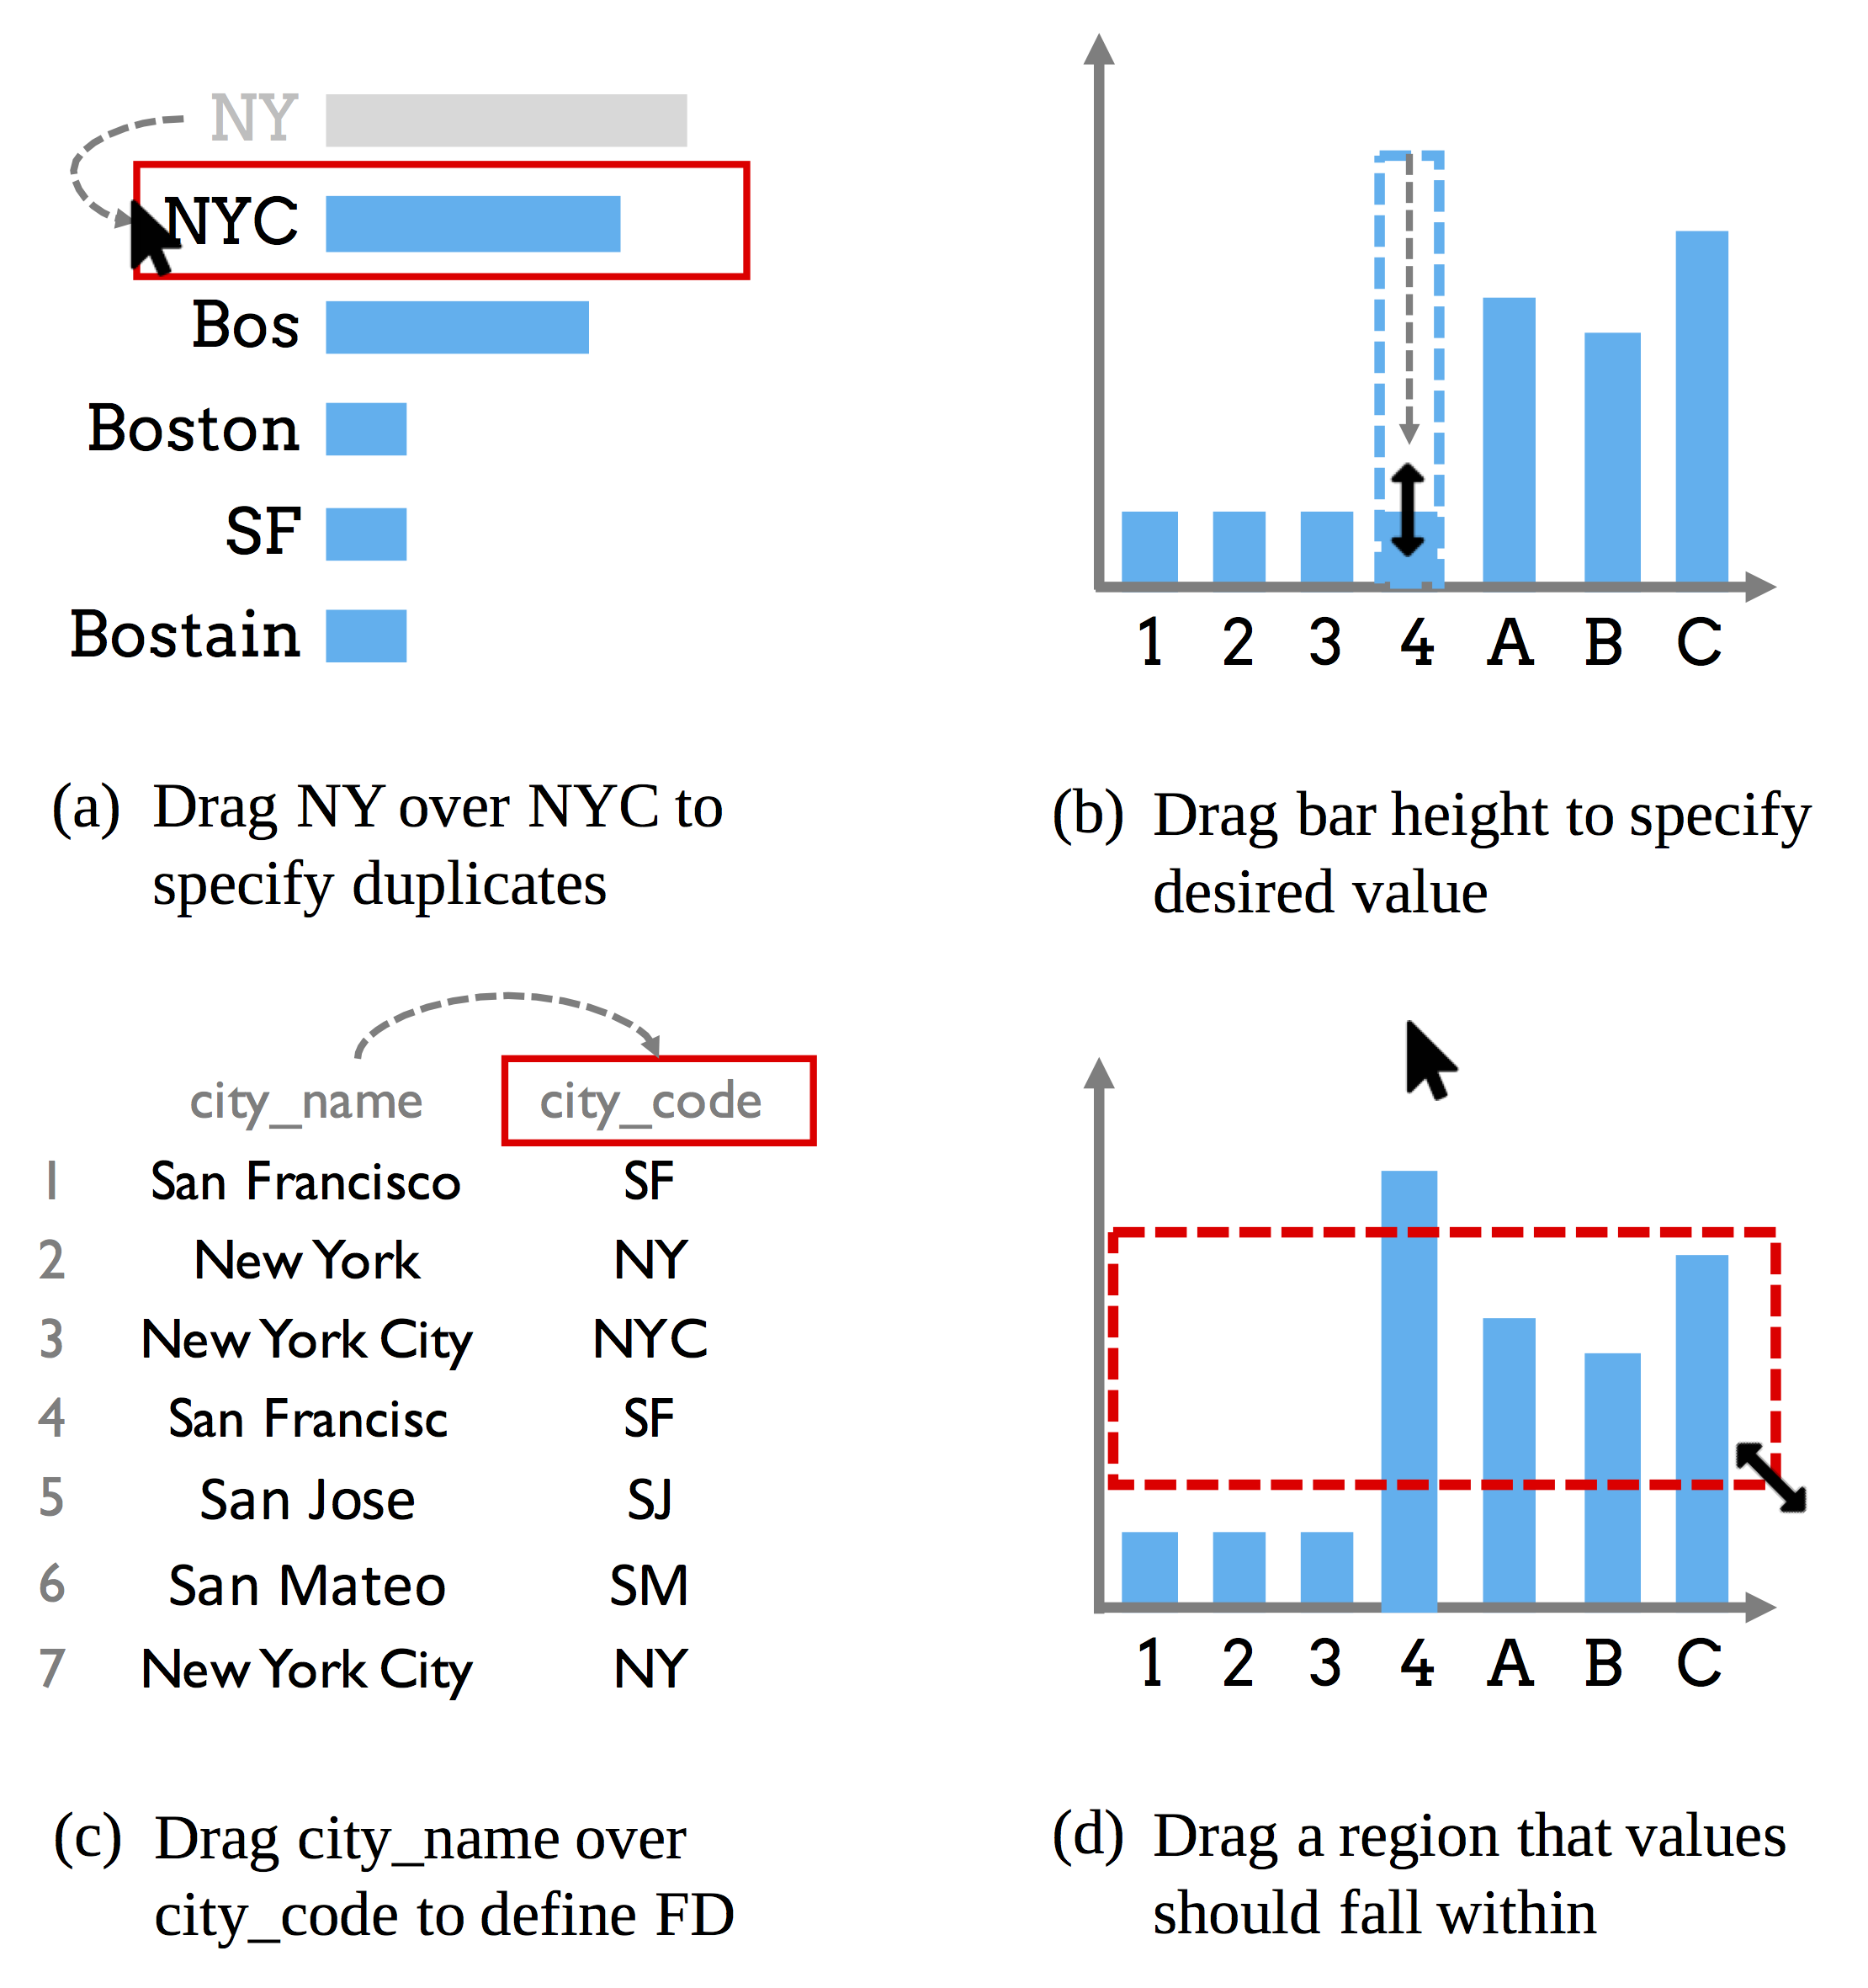
\includegraphics[width=.8\columnwidth]{figures/ui.png}
\label{f:ui}
\caption{Example interactions to specify visualization anomalies. \sys allows a user to specify complaints about a dataset in terms of an arbitrary scoring function and then searches over a language of transformations to best explain those complaints (i.e., what transformations remove them).}
\end{figure}

Going back to the terrorism dataset example, one key limitation of existing explanation engines is that they often only provide a partial explanation for why an aggregate is erroneous if there is dirty data in the mix. Predicate deletion may not be enough to explain output anomalies and may return a trivial or misleading result when there are errors. In Example~\ref{e:terrorism}, the dataset contains three classes of errors:  duplicates, zero-encoding rather than NULLs, and inconsistencies in location attributes. Rather than predicates that are \emph{correlated} with these anomalies, one would like to know suggested transformations that might make an anomalous aggregate typical--including setting values to defaults, merging entities, etc. 

An ideal explanation-enabled visualization interface would let the user interactively specify the anomalies within the visualization that rendered the anomalies, and allow an {\it explanation engine} to generate explanations in the form of succinct sequences of data transformations selected from an extensible library. Furthermore, it should be independent of the visual interface and detection model; effectively allowing for black box complaint specifications.

As a step towards this vision,  we present \sys, a transformation-oriented explanation engine that generalizes prior explanation engines along three dimensions---analysis program, anomaly types, and explanation language. 
\sys  provides a general API to generate explanations in the form of high-level transformation sequences for a wide range of anomalies that can be detected in an output visualization. Transformations are generated from an extensible library of parametrized data transformations.

Formally, \sys takes as input a {\it quality function} that scores each output record as a real-value between $[0,1]$ and a {\it language} of parameterized data transformation operators.  It uses a search-based algorithm to output a sequence of transformations (an explanation) from the language that seeks to maximize the quality function.  Similar to prior work~\cite{scorpion}, the quality functions can be derived from interactions in a visualization interface.  This API imposes minimal restrictions on the quality function, giving it tremendous flexibility regarding the data errors that it can express.   

Figure~\ref{f:ui} illustrates a number of examples: users can specify duplicates (a), incorrect values (b), functional dependencies and soft correlations (c), and threshold regions (d) through mouse-based interactions.   Using this, the user may generate a threshold rule that determines anomalous years in the terrorism dataset.   In this work, we focus on the core search problem, and assume the presence of a Python-based quality function.  We leave a detailed study of how to translate visualization-based interactions into quality functions as future work.  

The primary technical challenge is to quickly search the space of possible explanations.  This space is combinatorial in the possible transformation sequences as well as the possible parameterizations for each transformation in the sequence.  
To address this challenge, we make two key observations: 1) most errors are systematic in nature and their structure can be leveraged to reduce the search space, and 2) explanation generation can be cast as a planning problem, where the quality function is the objective and the explanation is the plan,  and leverage recent advances in robotics and reinforcement learning~\cite{dpm}.


\sys uses a best-first search that greedily appends data transformations to a set of best candidate programs seen so far, and adopts parallelization and pruning ideas from the search-based planning literature.  
In contrast to traditional search problems, where the search state (e.g., chess board) is compact and largely trivial to parallelize in a distributed setting, the data cleaning search state is the size of the input dataset and introduces a trade-off between communication costs to share intermediate state and the degree of parallelism possible.  
 To further accelerate its runtime, \sys can also encode problem-specific optimizations as search pruning rules (e.g., disallowed transformation sequences) or modifications to the data representation (e.g., clustering similar records).  
\sys also leverages the structure of systematic errors to adaptively learn prune rules during the search process, and estimate where or not candidate search branches will ultimately result in high-quality transformation sequences.  
 
The purpose of our experiments is to show the feasibility of a general search-based approach to explanation generation on real-world datasets and analyses.  To this end, we evaluate \sys on 8 real-world datasets used in prior data explanation and data cleaning literature. In each of these uses cases, we present different classes of quality functions and transformation languages--show that \sys is sufficiently general to address all of the domain specific challenges. 
In addition, we use synthetic datasets and errors to evaluate the precision, recall, and complexity of our proposed explanations in a controlled environment.  
We quantitatively evaluate \sys on its ability to generate accurate transformation rules in terms of accuracy on 7 real case studies. We create best effort pipelines for these case studies with existing systems and compare accuracies and runtimes.

% \sys certainly overlaps with data cleaning systems so we present comparisons when relevant.








\if{0}
\ewu{SANYAS TEXT BELOW}


% Detecting and handling dirty data is one of the most time-consuming steps of the data analysis process~\cite{nytimes}.
% It is often the case that such data is first identified by analysts during exploratory data analysis through visualizations or summary statistics that contain anomalous or otherwise unexpected values.

Predicates alone may not adequately explain all types of data anomalies.
Consider a dataset where both \texttt{New York} and \texttt{New York City} refer to the same \texttt{City} entity.
An analyst might detect an anomaly where a count aggregate is unexpectedly low for the group \texttt{New York}. 
A predicate explanation indicates that there exists a predicate, for example, \texttt{City = ``New York''}, that selects all of the anomalous values. 
However, this is only partial information--it tells the analyst nothing about the presence of the alternate entity \texttt{New York City}. 

In general, syntactic errors in a dataset are inherrently explained by data transformations--not just predicates.
It is desirable for the explanation engine to return a complete mapping rule, such as  \texttt{New York} $\rightarrow$ \texttt{New York City}, instead of just the predicate.
We can define a \emph{transformative explanation} as a minimal sequence of such rules from a formal language of rules such that after transformation the flagged values are no longer anomalous. 
Predicate explanations are a special-case of this framework, where the transformation rules are only deletions--in other words, identifying predicates to exclude from base data to remove a group of anomalous values.

\fi

% 
% It is widely known that data cleaning is one of the most time-consuming steps of the data analysis process~\cite{nytimes}, and
% designing algorithms and systems to automate or partially automate data cleaning continues to be an active area of research~\cite{DBLP:conf/sigmod/ChuIKW16}.
% Automation in data cleaning is challenging because real-world data is highly variable. 
% A single data set can have many different types of data corruption such as statistical outliers, constraint violations, and duplicates.
% Once an error is detected, there is a further question of how to repair this error, which often depends on how the data will be used in the future.
% 
% This variability creates a tension between generality and efficiency.
% While one might want a single cleaning framework that addresses all types of errors and repair operations, it is far more efficient to consider more specialized frameworks.
% Data cleaning tools are often highly optimized for particular problems  (e.g., see statistical outliers~\cite{hellerstein2008quantitative}, enforcing logical constraints~\cite{DBLP:conf/sigmod/ChuIKW16}, entity resolution~\cite{DBLP:journals/pvldb/KopckeTR10}). 
% Consequently, a recent survey of industry suggests that data cleaning pipelines are often a patchwork of custom scripts and multiple specialized systems~\cite{krishnan2016hilda}.
% The overhead to setup, learn, and manage multiple cleaning systems can easily outweigh the benefits.
% Some data scientists eschew automated tools altogether and simply write data cleaning programs from scratch.
% The customized programming approach quickly becomes difficult to mantain and interpret; especially for users without data engineering expertise~\cite{sculley2014machine}.
% 
% A single cleaning system that exposes a sufficiently flexible interface is clearly desirable; as long as the runtime and accuracy can be made comparable to existing alternatives.  
% To achieve this, we turn to the contemporary AI literature, which has produced exciting results such as AlphaGo~\cite{silver2016mastering} that were previously considered not possible.    This work shows that a combination of machine learning and massively parallelized search can effectively optimize highly complex objective functions.
% Our main observation is that data cleaning is very similar to the search problems considered in AI~\cite{russell1995modern}.
% The classic application is a computer chess program that must plan a sequence of chess moves that change the state of the board in order to maximize the likelihood of a checkmate. Likewise, in data cleaning, one is given a dirty relation and a way to measure data quality (e.g., number of integrity constraints violated), and the data cleaning problem is to find a sequence of modifications to the relation that maximize the data quality metric.
% 
% Most non-trivial problems are very hard without good search heuristics.
% Advances in machine learning have made it possible to replace hand-crafted heuristics with automatically learned pruning functions that estimate the expected quality of candidate plans. AlphaGo learned pruning heuristics using a neural network trained on data generated through self-play~\cite{silver2016mastering}.
% This insight is highly relevant to data cleaning, where datasets tend to have structure amenable to learning heuristics adaptively.
% Data errors are often systematic where they are correlated with with certain attributes and values in the dataset~\cite{rekatsinas2017holoclean,DBLP:journals/pvldb/KrishnanWWFG16}.
% Consequently, as more data is cleaned, we can better identify common patterns to prioritize the search on future data.
% We may not necessarily need a neural network for data cleaning, but the overall algorithmic structure of AlphaGo, tree-search combined with a learned heuristic, can be very useful.
% 
% \sys is a new data cleaning system that is designed around a search-based model. It takes as input a {\it quality function} that models the data quality of a relation as a real-value between $[0,1]$ and a {\it language} of parameterized data cleaning operators, and outputs a sequence of data cleaning transformations (a cleaning program) from the language that seeks to maximize the quality function.This API imposes minimal restrictions on the quality function, giving it tremendous flexibility in terms of the data errors that it can express.   As a comparison, a recent system called Holoclean~\cite{rekatsinas2017holoclean} is similar in that it provides a rich interface to specify denial constraints and lookup tables, and integrates them within a probabilistic model to more accurately resolve constraint violations.  In contrast, \sys's quality function is a user-defined function that can express {\it arbitrary combinations} of denial constraints {\it as well as} statistical, quantitative, text formatting, and other classes of data errors.  For instance, \Cref{s:expquant} shows how \sys can perform cleaning for machine learning applications by embedding machine learning training and evaluation within the quality function, while \Cref{s:expterror} combines entity resolution, outlier cleaning, and functional dependency violations within the same function.  
% 
% 
% \sys uses a best-first search that greedily appends data transformations to the set of best candidate programs seen so far, and adopts parallelization and pruning ideas from the search-based planning literature.  In contrast to traditional search problems, where the search state (e.g., chess board) is compact and largely trivial to parallelize in a distributed setting, the data cleaning search state is the size of the input dataset and introduces a trade-off between communication costs to share intermediate state and the degree of parallelism possible.  
% To further accelerate its runtime, \sys can also encode problem-specific optimizations as search pruning rules (e.g., disallowed transformation sequences) or modifications to the data representation (e.g., clustering similar records).  We find that many optimizations in existing cleaning systems may be cast as search pruning rules.
% 
% \sys can adaptively learn pruning rules to avoid unprofitable search branches during the search process.
% While AlphaGo used a deep neural network and massive amounts of training data to model the heurisitic, we found that a simple logistic regression classifier and training data gathered during the search process was sufficient to reduce the runtime by multiple orders of magnitude. 
% It is important to acknowledge that \sys loses many of the provable guarantees provided by specialized systems based on logical constraints, and is in some sense, best-effort.  
% Across 8 real-world datasets used in prior data cleaning literature, we show that \sys matches or exceeds the cleaning accuracy and exhibits competitive run-times to state-of-the-art approaches that are specialized to a specific error domain (constraint, statistical, or quantitative errors).  
% 
% \subsection{Main Benefits}
% \begin{itemize}[leftmargin=*, topsep=0mm, itemsep=0mm]
% \item \stitle{Optimization} Existing cleaning pipelines must combine disparate cleaning solutions and manage glue code to transfer data between systems.  However, data transfer can be a non-trivial portion of the total cleaning cost and recent work~\cite{palkar2017weld} has shown that a common runtime can avoid data movement and improve runtimes by up to $30\times$.  
% 
% \item \stitle{Generalization and Robustness} In contrast to existing cleaning systems, that output a cleaning relation, \sys outputs a composable cleaning program that is both simpler to understand because it groups common fixes together, and can be applied to new data.  In addition, the cleaning program allows us to analyze cleaning systems for overfitting.  We indeed find that the complexity of the quality function and cleaning language can lead to overfitting, and believe this is the case for any data cleaning system.  We also show that simple changes to the quality function can act as regularization terms to control the degree of overfitting.
% 
% \item \stitle{Software Engineering}  Users do not need to write and manage glue code; do not need to manage ETL between systems; and do not need to learn system specific abstractions, languages, and assumptions.  All of these are arguably intangible, but critical friction points in the highly iterative cleaning process.  
% 
% \item \stitle{New Cleaning Applications} We envision that a single API makes it possible to support an ecosystem of domain-specific cleaning specification libraries.  For instance,  interactive visualization interfaces akin to~\cite{trifacta,kandel2011wrangler,DBLP:journals/pvldb/0002M13,wu2012demonstration} can directly translate user interactions into a wide range of cleaning constraints.   
% \end{itemize}
% 
% 
% 
% 
% % * single library/language with the same abstraction is important (software engineering)
% %   * no more glue code -- talk about weld, etc.  
% %   * no ETL between systems
% %   * no leraning new abstractions
% %   * new languages to specify constraints and quality goals.  some are languages, some are APis, some are systems
% %   * engineering: systems like llunatic, need to satisfy postgres schema to get started
% % 
% % * different
% %   * application driven cleaning by embedding downstream app into the quality function
% %   * new apps
% %     * viz stuff needs a single api
% %     * mixed datasets -- numeric and relational data
% %     * many interfaces to compose and create quality functions and languages
% % 
% % * holoclean
% %   * lets them express denial constraints and use a knowledge base to decide how to resolve violations
% %   * we suppor denial constraints, as well as numeric errors, text extraction errors, and arbitrary formulations of teh quality measure.  
% % 
% % 
% % * unification -->
% %   * reduces engineering to implement cleaning system
% %   * joint optimization if overlapping in 
% % * generalize to new data 
% %   * overfitting
% % * parallelize opportunities
% 
% 
% 
% 
% 
% 
% 
% 
% 
% 
% 
% 
% \if{0}
% Data cleaning usually involves tedious manual specification of transformation rules.
% For example, a data scientist might write a rule that maps every record with a \textsf{country} attribute ``United States'' to ``United States of America''.
% These collections of rules quickly grow in size, and if they are developed in an ad-hoc way, they can be brittle and hard to maintain~\cite{krishnan2016hilda}.
% Overly specific rules may not apply to future data, and overly general rules, might introduce unwanted side-effects.
% Designing accurate transformation rules is a painstaking process, which is widely reported to be one of the most effort-intensive steps in data science~\cite{nytimes}.
% 
% We explore to what extent such transformation rules can be learned through a process of automatic trial-and-error on a dataset.
% The system simulates different sequences of data transformations and scores the result according to a user-specified data quality objective function.
% On its own, this is an inefficient way to search to search the set of transformation rules.
% However, we can leverage Machine Learning to learn a strong pruning heuristic incrementally.
% Transformations are often parametrized by literal values from the database (e.g., find string X and replace with string Y).
% If we clean data in small partitioned blocks, we can incrementally build a classifier that infers common patterns in these literals, such as whether the strings tend to be similar or tend to be different or the attributes that are likely to be touched.
% For example, consider the problem above where a data scientist is resolving inconsistencies in a \textsf{country} attribute to satisfy an integrity constraint.
% As we iterate through the distinct \textsf{country} values and simulate possible replacement values, it might become clear that the source string have to be close to the target strings in string similarity, i.e., ``United States'' is more likely to be replaced by ``United States of America'' than ``Zimbabwe''.
% Learning such a relationship automatically avoids hand coded heuristics which have to consider the complex relationship between how the analyst describes data quality and how exactly the transformations are defined.
% 
% This basic algorithm, optimizing a sequence of black-box transformations over a black-box data quality function, has a number of important advantages: (1) it is highly expressive as it can model a wide range of data cleaning formalisms from integrity constraints to quantitative data cleaning in the same framework, (2) it is relatively easy to parallelize the search, and (3) the result of the algorithm is not only a cleaned database instance but transformations that can be applied to future data.
% This formalism casts data cleaning as a planning problem; analogous to the algorithms used AI, Robotic Planning, and Control.
% Similar to the way one plans out a sequence of chess moves in AI to gain a strategic board position, we can think of data cleaning as planning out a sequence of data transformations to maximize the score on a data quality function.
% And as in chess, where one cannot perfectly anticipate the opposing player's moves, in data cleaning we may not have a strong \emph{a priori} model of how a user-defined transformation rule modifies the data.
% As a result, the algorithm and search heuristics cannot make strong assumptions about the anticipated structure of any search instance.
% This sort of an approach is increasingly attractive because recent results in AI demonstrate scaling these search problems to  high branching-factor domains even when few assumptions are made.
% Recent algorithms have been shown to match or exceed human performance in domains such as Go~\cite{silver2016mastering} and in Atari video games~\cite{mnih2015human}.
% As in many classical data cleaning problems, an optimal solution to AI search problems is very hard to discover, but pragmatically leverage distributed computing and pruning rules learned from data can tractably find acceptable solutions.
% 
% We use this algorithm as a starting point for a new data cleaning system called \sys.
% We designed an API that takes classical data cleaning problem specifications, such as integrity constraints, gold-standard manually cleaned data, and statistical models, and translates those specifications into an iterative learning search problem. 
% Of course, we often need special-case optimizations that prune unproductive search branches to make the runtime more competitive with special case systems.
% We provide a model where pruning rules are specified as regular expressions over a formal language of transformations and can be static (i.e., fixed before execution) and dynamic (i.e., inferred from properties of the dirty database instance).
% The search algorithm we use is a memory-bounded best-first search which maintains the subset of the search frontier that can fit in memory. 
% This algorithm can be parallelized, distributed, and can cache repeated computations.
% \fi
% 
% 
% 
% \if{0}
% 
% 
% view data cleaning from a planning~\cite{} and optimization perspective, and show evidence that a simple, general approach to this problem can provide the user with considerable flexibility in terms of cleaning data with different classes of errors, controlling the allowable operations, and customizing the system to new types of data errors.
% 
% 
% 
% Ideally, the majority of the data cleaning process should reside in a single system with a  \emph{declarative} interface, wherein the analyst specifies a high-level data model (e.g., constraints the data should satisfy) and a system automatically generates the pipeline to enforce the model.
% The idea of declarative data cleaning is not new~\cite{rahm2000data}, but such approaches have classically been restricted to data models specified in subsets of first-order logic and only recently have considered extensions better handle uncertain numerical data~\cite{prokoshyna2015combining}.
% The prevailing wisdom is that there is an inherent tradeoff between the expressiveness of the data model and the efficiency of the (approximate) solution algorithm---limited models allow the system designer to exploit specific algorithmic structures.
% 
% 
% However, two recent trends, namely, the success of model-free learning in AI and the availability commodity cloud computing encourage us to reconsider this algorithmic philosophy.
% Recent progress in planning problems such as AlphaGo~\cite{silver2016mastering} and automatically playing Atari video games~\cite{mnih2015human} have shown that a prudent combination of Machine Learning and distributed search can approximately optimize very complex black-box objective functions.
% The intriguing aspect of these results is that the same algorithm, called Deep Q Reinforcement Learning, that learns to play an Atari game~\cite{mnih2015human} can be used on a very different problem, such as training a robot~\cite{gu2017deep}.
% The underlying optimization algorithm encodes few specifics about the objective or structure of the domain  and pragmatically finds a reasonable local optimum.
% The optimization algorithm is general enough to support a very wide class of problems--at the cost of additional computational resources since it is unaware of instance-specific structure.
% 
% \fi

\section{Related Work}

\ewu{what is different from data cleaning? and why you shouldn't use a cleaning system for explanations and call it a da}


\ewu{Argue that existing data cleaning systems each support a limited type of quality function and transformation language.  Holoclean  does not support arbitrary transformation templates }


Data cleaning is nearly as old as the relational model~\cite{codd1970relational}, and numerous research and  commercial systems have been proposed to improve data cleaning efficiency and accuracy (see~\cite{rahm2000data} for a survey and \Cref{s:probexpressiveness} for related systems).
The recent advances in scalable data cleaning~\cite{wang1999sample, DBLP:journals/debu/KrishnanWFGKM015, khayyat2015bigdansing, altowim2014progressive} has revealed {\it human-time}---finding and understanding errors, formulating desired characteristics of the data, writing and debugging the cleaning pipeline, and basic software engineering---as a dominant bottleneck in the entire data cleaning process~\cite{krishnan2016hilda}.  
\sys aims to address this bottleneck by using the quality function and transformation language as a flexible and expressive declarative interface to separate high level cleaning goals from how the goals are achieved.   

%However, \emph{machine time} is only part of the story and the \emph{human time} of data cleaning is known to be significant.  \sys aims to reduce the human time in writing data cleaning scripts by allowing the data scientist to model the data at a high-level and the system searches for the appropriate low-level transformations.  

%\stitle{Automatic Data Cleaning}  Automatic cleaning systems express data errors as violations of logical constraints and seek to edit the database in a way to resolve such violations.  The Chase~\cite{aho1979theory,maier1979testing} serves as the basis of 

\stitle{Machine Learning in Data Cleaning} Machine learning has been widely used to improve the efficiency and/or reliability of data cleaning~\cite{DBLP:journals/pvldb/YakoutENOI11,yakout2013don,gokhale2014corleone}.
It is commonly used to predict an appropriate replacement attribute value for dirty records~\cite{yakout2013don}.
Increasingly, it is used in combination with crowd-sourcing to extrapolate patterns from smaller manually-cleaned samples~\cite{gokhale2014corleone,DBLP:journals/pvldb/YakoutENOI11} and to improve reliability of the automatic repairs~\cite{DBLP:journals/pvldb/YakoutENOI11}.
Concepts such as active learning can be leveraged to learn an accurate model with a minimal number of examples~\cite{DBLP:journals/pvldb/MozafariSFJM14}.
Recently, HoloClean~\cite{rekatsinas2017holoclean} uses probabilistic graphical models to combine multiple quality signals such as lookup tables and constraints to predict cell-level repairs.
Although related, \sys uses machine learning to steer the search process {\it away} from low quality candidate programs, rather than to propose ideal cleaning programs.  From this perspective, \sys can be extended to leverage ideas from existing work to steer the search process {\it towards} promising programs.  

% For example, Yakout et al. train a model that evaluates the likelihood of a proposed replacement value \cite{yakout2013don}.
% Another application of machine learning is value imputation, where a missing value is predicted based on those records without missing values.
% Machine learning is also increasingly applied to make automated repairs more reliable with human validation \cite{DBLP:journals/pvldb/YakoutENOI11}.
% Human input is often expensive and impractical to apply to entire large datasets.
% Machine learning can extrapolate rules from a small set of examples cleaned by a human (or humans) to uncleaned data \cite{gokhale2014corleone, DBLP:journals/pvldb/YakoutENOI11}.
% This approach can be coupled with active learning \cite{DBLP:journals/pvldb/MozafariSFJM14} to learn an accurate model with the fewest possible number of examples.
% Holoclean~\cite{rekatsinas2017holoclean} leverages machine learning to validate repairs with a probabilistic graphical model.
% \sys uses machine learning in the synthesis process to prune search branches.


\stitle{Application-Aware Cleaning}  Semantics about the downstream application can inform ways to clean the dataset ``just enough'' for the application.  
A large body of literature addresses relational queries over databases with errors by focusing on specific classes of queries~\cite{altwaijry2015query}, leveraging constraints over the input relation~\cite{2011Bertossi}, integration with crowd-sourcing~\cite{DBLP:conf/sigmod/BergmanMNT15}.   Recent work such as ActiveClean~\cite{DBLP:journals/pvldb/KrishnanWWFG16} extend this work to downstream machine learning applications, while Scorpion~\cite{DBLP:journals/pvldb/0002M13} uses the visualization-specified errors to search for approximate deletion transformations.   In this context, \sys can embed application-specific cleaning objects can be modeled within the quality function.  For instance, our quantitative cleaning experiments (\Cref{s:expquant}) simply embeds the model training and accuracy computation in the quality function. 
There has also been recent work on quantifying incompleteness in data quality metrics~\cite{chung2016data}.

% For example, Altwaijry et al.~\cite{altwaijry2015query} describe a technique for resolving a sufficient subset of entities in a database to answer SPJ queries.
% Bergman et al. \cite{DBLP:conf/sigmod/BergmanMNT15} proposed identifying errors in selection query results and generating crowd-scoured queries to determine fixes to the base data.
% Similarly, work on the consistent query answering problem explored the minimal effort needed to answer a query given a set of integrity constraints over a dirty relation~\cite{2011Bertossi}.
% While the work on relational queries is extensive, analytical queries (aggregates, advanced statistical analytics, learning etc.) is less studied.
% Projects like ActiveClean~\cite{DBLP:journals/pvldb/KrishnanWWFG16} have studied algorithms for prioritizing user-defined cleaning using the downstream ML model.
% \sys is a flexible framework where such cleaning objectives can be modeled easily as different quality functions.

% There is a growing body of literature that studies analysis-driven data cleaning, that is, applying data cleaning in a sufficient way to answer a given query (defining quality flexibly as the accuracy of the query result).

\stitle{Generating Cleaning Programs} A composable data cleaning language is the building block for systems like \sys that generate understandable cleaning programs.   Languages for data transformations have been well-studied, and include seminal works by Raman and Hellerstein~\cite{raman2001potter} for schema transformations and Galhardas et al.~\cite{DBLP:conf/vldb/GalhardasFSSS01} for declarative data cleaning. These ideas were later extended in the Wisteria project~\cite{DBLP:journals/pvldb/HaasKWF015} to parametrize the transformations to allow for learning and crowdsourcing.   Wrangler~\cite{wrangler} and Foofah~\cite{jin2017foofah} are text extraction and transformation systems that similarly formulate their problems as search over a language of text transformations, and develop specialized pruning rules to reduce the search space.   These can be viewed as special cases of \sys.




\section{Problem Definition}
This section presents the basic \sys formalisms and our relationship to related work.

\subsection{Data Transformations}
We focus on data transformations that concern a single relational table. 
Let $R$ be a relation over a set of attributes $A$,  $\mathcal{R}$ denote the set of all possible relations over $A$, and $r.a$ be the attribute value of $a \in A$ for row $r \in R$.
A data transformation $T(R): \mathcal{R} \mapsto \mathcal{R}$ maps an input relation instance $R \in \mathcal{R}$ to a new (possibly cleaner) instance $R' \in \mathcal{R}$ that is union compatible with $R$.  For instance, ``replace all \texttt{city} attribute values equal to {\it San Francisco} with {\it SF}'' may be one data transformation, while ``delete records where \texttt{city} is {\it SF}'' may be another.   
Aside from union compatibility, transformations are simply UDFs.

%We find that nearly all cleaning transformations in existing literature satisfy these properties \ewu{(See Appendix of technical report)}. 

Data transformations can be composed using the binary operator $\circ$ as follows: $(T_i \circ T_j)(R) =  T_i(T_j(R))$.
The composition of one or more data transformations is informally called an {\it explanation}, and more formally called a {\it transformation program} $p$.   If $p = p' \circ T$, then $p'$ is the parent of $p$; the parent of a single data transformation is a NOOP.  In practice, users will specify {\it transformation templates} $\mathbb{T}(\theta_1,\cdots,\theta_k)$, and every assignment of the parameters represents one possible transformation.  
Although $\mathbb{T}$ can in theory be an arbitrary deterministic template function, our current implementation makes several simplifying assumptions to bound the number of data transformations that it can output.  We assume that a parameter $\theta_i$ is typed as an attribute or a value.  The former means that $\theta_i$'s domain is the set of attribute names in the relation schema; the latter means that $\theta_i$'s domain is the set of cell values found in the relation, or otherwise provided by the user. 

\begin{example}\label{ex1}
The following \texttt{City} relation contains two attributes \textsf{city\_name} and \textsf{city\_code}.  Suppose there is a one-to-one relationship between the two attributes. In this case, the relation is inconsistent with respect to the relationship and contains errors highlighted in \red{red}.

  \begin{table}[ht!]
	\small
  \centering
  \label{my-label}
  \begin{tabular}{|l|l|l|}
  \hline
  \rowcolor[HTML]{000000} 
  & \white{city\_name}            & \white{city\_code}   \\ \hline
  1 & San Francisco                    & SF                                  \\ \hline
  2& \red{\textbf{New York}}           & NY                                  \\ \hline
  3 & New York City                    & \red{\textbf{NYC}} \\ \hline
  4 & \red{\textbf{San Francisc}}      & SF                                  \\ \hline
  5 & San Jose                         & SJ                                  \\ \hline
  6 & San Mateo                        & SM                                  \\ \hline
  7 & New York City                    & NY                                  \\ \hline
  \end{tabular}
  \end{table}

The following transformation template uses three parameters: \texttt{attr} specifies an attribute, \texttt{srcstr} specifies a source string, and \texttt{targetstr} specifies a target string.   
{\small\[
T = \textsf{find\_replace}(\text{srcstr}, \text{targetstr}, \text{attr})
\]}
The output of the above is a transformation $T$ that finds all \texttt{attr} values equal to \texttt{srcstr} and replaces those cells with \texttt{targetstr}. 
For instance, \texttt{find\_replace(``NYC'', ``NY'', ``city\_code'')(City)} returns a data transformation that finds records in \texttt{City} whose city\_code is ``NYC'' and replaces their value with ``NY''.
\end{example}


Let $\Sigma$ be a set of distinct data transformations $\{T_1,\cdots,T_N\}$, and
$\Sigma^*$ be the set of all finite compositions of $\Sigma$, i.e., $T_i\circ T_j$.
A formal language $L$ over $\Sigma$ is a subset of $\Sigma^*$.
A program $p$ is valid if it is an element of $L$.

\begin{example}\label{ex2}
  Continuing \Cref{ex1}, $\Sigma$ is defined as all possible parameterizations of \texttt{find\_replace}.  Since many possible possible parameterizations are non-sensical (e.g., the source string does not exist in the relation), we may bound $\Sigma$ to only source and target strings present in each attribute's instance domain (a standard assumption in other work as well~\cite{DBLP:series/synthesis/2012Fan}).  In this case, there are $61$ possible data transformations, and $\Sigma^*$ defines any finite composition of these $61$ transformations.  The language $L$ can be further restricted to compositions of up to $k$ data transformations.  
\end{example}

Finally, let $Q(R): \mathcal{R} \mapsto [0,1]$ be a quality function where $1$ implies that the instance $R$ has no anomalies, and a lower value correspond to a more anomalies table.
Since running a program $p\in\mathcal{L}$ on the initial dirty table $R_{dirty}$ returns another table, $Q(p(R_{dirty}))$ returns a quality score for each program in the language.  
$Q$ is a UDF and we do not impose any restrictions on it. In fact, one experiment embeds training and evaluating a machine learning model {\it within} the quality function (\Cref{s:expquant}).  Another experiment shows that \sys can be robust to random noise injected in the function (\Cref{s:expoverfit}).   

Even so, we call out two special cases that provide optimization opportunities. 
We define two sub-classes of quality functions: row-separable and cell-separable quality functions.
The former expresses the overall quality based on row-wise quality function $q(r): R \mapsto [0,1]$ where $1$ implies that the record is clean:
$Q(R) \propto \sum\nolimits_{r \in R} q(r)$
Similarly, a cell-separable quality function means that there exists a cell-wise quality function $q(r, a): (R\times A) \mapsto [0,1]$, such that the quality function is the sum of each cell's quality: 
$Q(R) \propto \sum\nolimits_{r \in R} \sum_{a \in A} q(r,a)$.

These special cases are important because they can define hints on what types of transformations are irrelevant.
For example, if the quality function is cell-separable, and we have identified that a set of cells $C$ are dirty (e.g., they violate constraints), then we can ignore transformations that do not modify cells in $C$.  This restricts the size the language and makes the problem much easier to solve.


\noindent We are now ready to present data cleaning as the following optimization problem:
\begin{problem}[$\textsf{clean}(Q,R_{dirty},L)$]
Given quality function $Q$, relation $R_{dirty}$, and language $L$, find valid program $p^* \in L$ that optimizes $Q$:
\[
p^* = ~ \max_{p \in L} Q( p(R_{dirty}) ).  
\]
\end{problem}
$p^*(R_{dirty})$ returns the cleaned table, and $p^*$ can be applied to any table that is union compatible with $R_{dirty}$.
A desirable property of this problem formulation is that it directly trades off runtime with cleaning accuracy and can be stopped at any time (though the cleaning program may be suboptimal).  At the limit, \sys simply explores $L$ and identifies the optimal program.


\begin{example}\label{ex3}
Continuing~\Cref{ex1}, let us assume the following functional dependencies over the example relation: $\textsf{city\_name} \rightarrow \textsf{city\_code}$ and $\textsf{city\_code} \rightarrow \textsf{city\_name}$.
We can efficiently identify inconsistencies by finding the cities that map to $>1$ city code, and vice versa.   Let such city names and codes be denoted $D_{city\_name}$ and $D_{city\_code}$, respectively.
$Q(R)$ is a cell-separable quality function where the cell-wise quality function is defined as $q(r, a) = 1 - (r.a \in D_a)$, such that $r.a$ is $1$ if the attribute value does not violate a functional dependency, and $0$ otherwise.

By searching through all possible programs up to length 3 in $L$, we can find a cleaning program based on \texttt{find\_replace} that resolves all inconsistencies:
\begin{lstlisting}
    find_replace(New York, New York City, city_name)
    find_replace(San Francisc, San Francisco, city_name)
    find_replace(NYC, NY, city_code)
\end{lstlisting}
\end{example}


\subsection{Problem Expressiveness}\label{s:probexpressiveness}

\subsection{Case Studies}
\textbf{TODO}

\subsection{Approach Overview and Challenges}
Our problem formulation is a direct instance of {\it planning} in AI~\cite{russell1995modern}, where an agent identifies a sequence of actions to achieve a goal.  In our setting, the agent (\sys) explores a state space ($\mathcal{R}$) from an initial state (the input relation) by following transitions (applying $T_i \in \Sigma$) such that the sequence of actions is valid (within $\Sigma^*$) and the quality of the final state ($Q(R_{final})$) is maximized.  

For readers familiar with stochastic processes, this search problem is equivalent to a deterministic Markov Decision Process (MDP), where the states are $\mathcal{R}$, the actions $\Sigma$, the transition function updates the instance with the transformation, the initial state is the dirty instance $R_{dirty}$, and the reward function is $Q$.

One may be hesitant in adopting our problem formulation because, although it is sufficiently general to model many existing data cleaning problems, such generality often comes at the expense of runtime performance.   The planning problem is known to be APX-Hard, meaning there does not exist a polynomial time approximation unless P=NP.  
% Let $R$ be a single-attribute relation of Booleans. Let $L$ be the set of all assignments to a single value.  Given a list of $N$ Boolean clauses over all the boolean variables, let $Q$ assign to each record one minus the fraction of clauses that evaluate to true. This formulation is equivalent to MAX-SAT and solution to the optimization problem. 

Despite the problem's worst-case complexity, 
recent successes in similar planning problems---ranging from AlphaGo~\cite{silver2016mastering} to automatically playing Atari video games~\cite{mnih2015human} have shown that a prudent combination Machine Learning and distributed search can find practical solutions by leveraging the structure of the problem. 
Not every problem instance is as pathological as the worst case complexity suggests, and there are many reasonable local optima.









\if{0}
    Every data cleaning problem in \sys is specified by a deterministic finite automaton (DFA). 
    A DFA is a 5-tuple:
    \[\langle S, A, \delta, s_0\rangle,\]
    where $S$ is a set of states that the process can be in, $A$ is a set of inputs that the process can take, $\delta$ is a transition function that takes as input a state and an input and transitions the process to the next state in $S$, and $s_0$ is an initial state of the process.

    The set of relations and the language of transformations defines a DFA:
    \[\langle \mathcal{R}, \Sigma, \delta, R_{dirty}\rangle, \]
    where the states $\mathcal{R}$ is the set of possible instances, the inputs are transformations from $\Sigma$, the transition function updates the instance with the transformation, and the initial state is the dirty instance $R_{dirty}$. Search problems can be defined over the DFA. 
    A quality function $Q$ maps an instance $R$ to a scalar where 1 implies it is clean:
    \[
    Q: \mathcal{R} \mapsto [0,1]
    \]
    A separable quality function is one that can be expressed as an average over cell-wise quality metrics $q(r,a)$ where 1 implies clean:
    \[
    Q(R) \propto \sum_{r \in R} \sum_{a \in A} q(r,a)
    \]

    Note that in contrast to traditional programming-by-example problems~\cite{}, which take as input a well defined input and goal state, the latter is not present in our problem formulation.  It is replaced with a quality function that we seek to maximize.  This is an important distinction because (1) it models the uncertain nature of data cleaning, where the ground truth is typically not available~\cite{}, and (2) necessarily greedy.

    \vspace{0.5em} \noindent \textbf{Remark 1: } 



\fi








\section{Architecture and API}

\begin{figure}[t]
% \vspace{-5pt}
\centering
 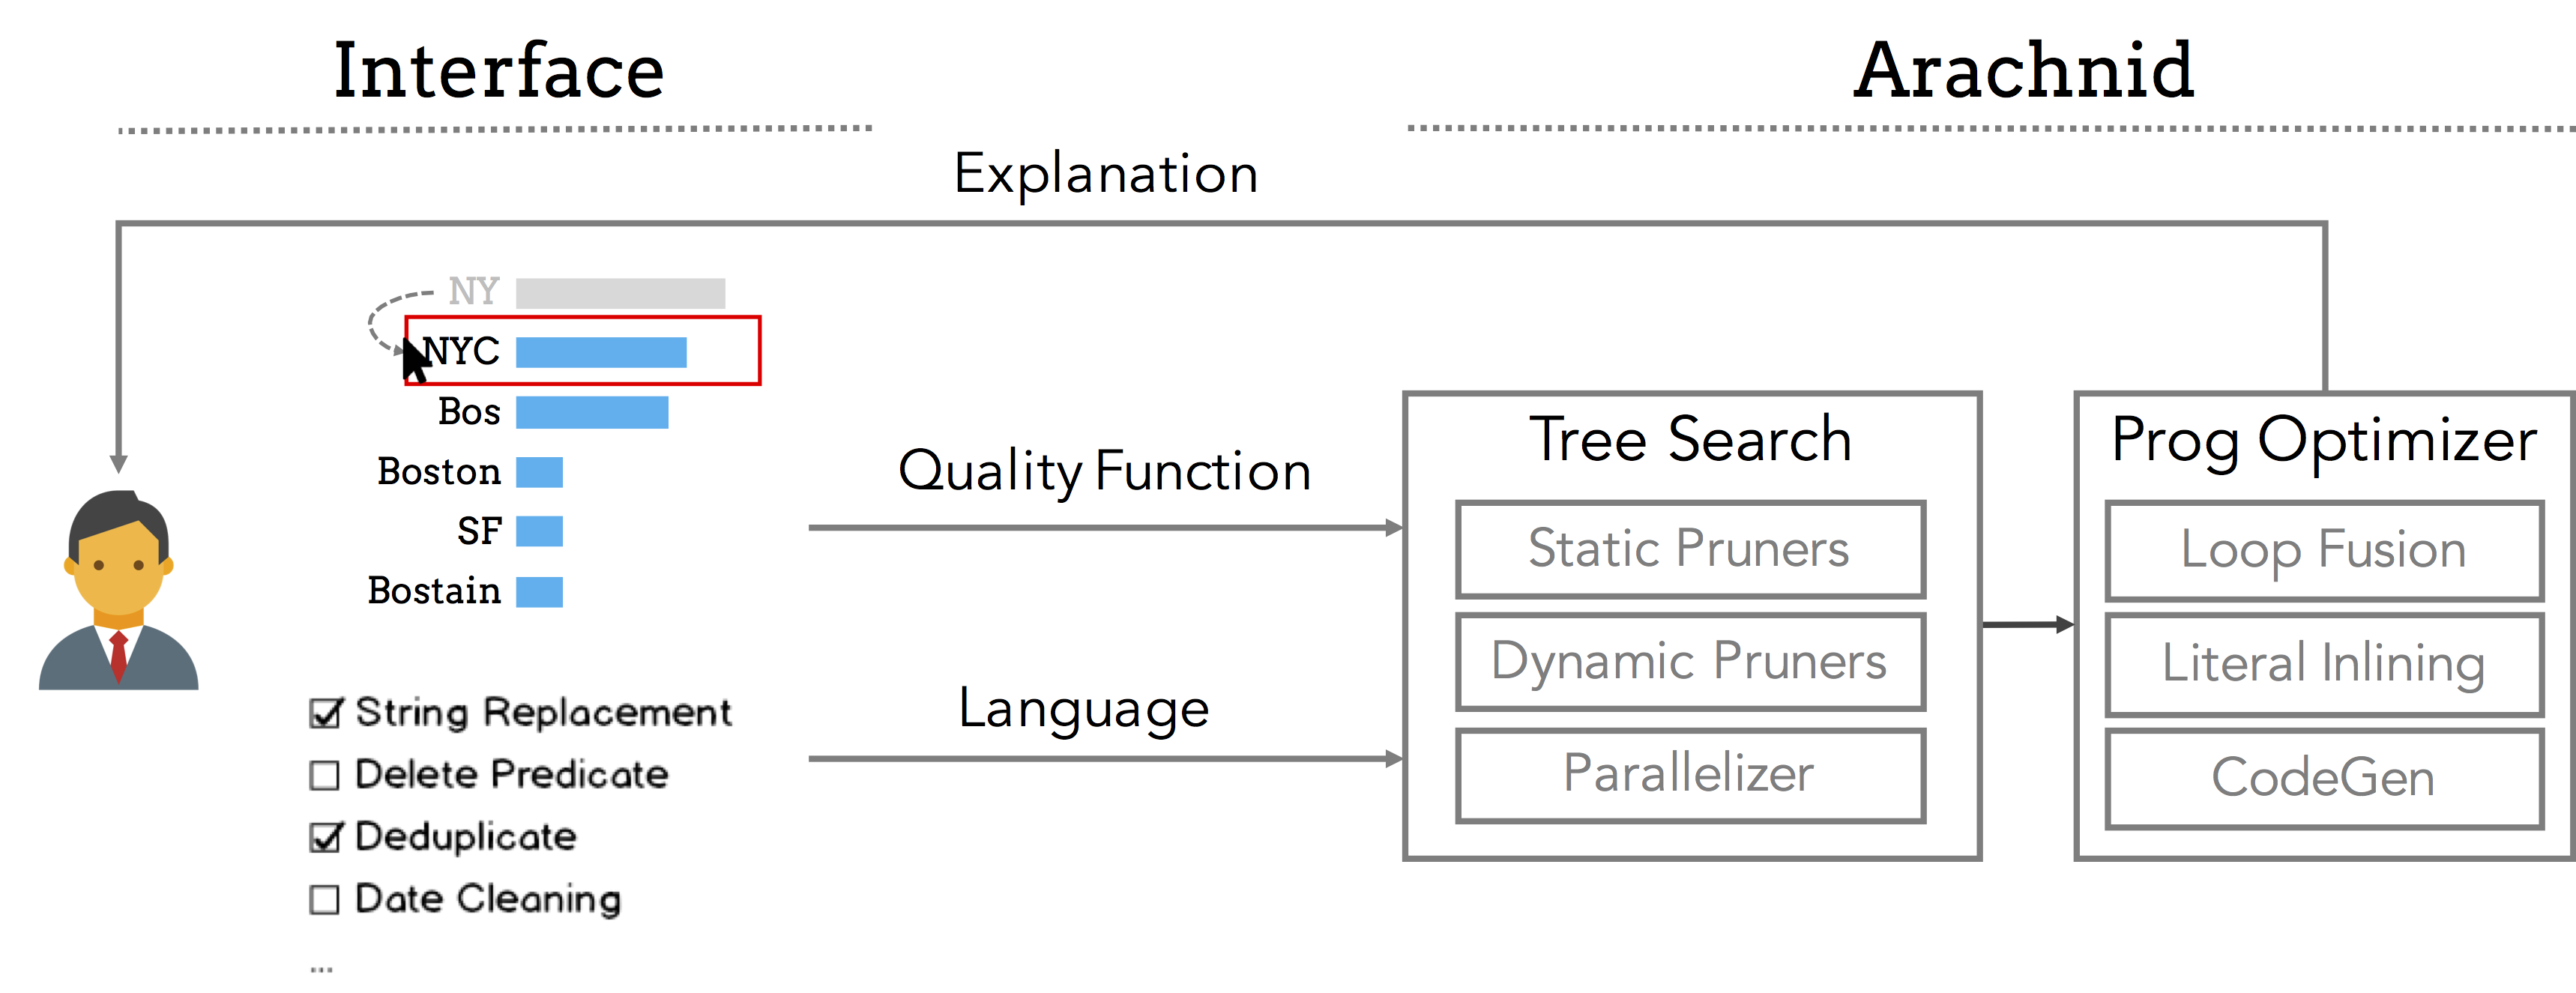
\includegraphics[width=\columnwidth]{figures/arachnidarch.png}
 \caption{\small Arachnid architecture.  Users interactively specify quality functions through the visualization, and optionally select transformation templates. \sys uses an optimized tree search to find and optimize a sequence of transformations (explanation) to maximize the quality measure.   \label{fig:arch} }

\end{figure}
% This section describes the three major components of the \sys system architecture (\Cref{fig:arch}), split between the user interface to specify the cleaning problem, the core search algorithm, and optimization of the resulting cleaning program.  We detail the interface and program optimization in this section, and focus on the search algorithm and optimizations in the rest of the paper. Designing data cleaning interfaces~\cite{DBLP:conf/uist/GuoKHH11} and query optimization for data cleaning~\cite{DBLP:conf/vldb/GalhardasFSSS01, khayyat2015bigdansing} are interesting problems in their own right, and we believe \sys can enable simpler and more powerful approaches.  However, these were not a focus of the current study.

The {\it Client Interface} allows the user to interactively specify anomalies through drag-and-drop interactions and lightweight text annotations (Figure~\ref{f:ui}).   These interactions are translated into a Python quality function $Q$.  Alternatively, the user can write the quality function directly.    The interface also provides a list of common transform templates in case the user wants to deselect any that are not applicable to her domain.  She may similarly write her own parameterized transformation template.  These are used to specify the transformation language $L$.

% contains extensible libraries of domain-specific quality functions, cleaning data transformations, and pruning feature hints that the user can use to define a high level cleaning goal.  Our current implementation can translate a wide range of domain-specific goals---including type constraints, functional dependencies, denial constraints, lookup tables, parametric and non-parametric outlier models, and correlations between numeric attributes---into a single quality function.  Users can also constrain the cleaning language, and we currently support any type of conditional cell and record transformation that applies a black-box transformation to all cells or records satisfying a predicate; both the transformation parameters and the predicate are learned by \sys.  Finally, users can optionally provide features that \sys uses to dynamically learn pruning rules (Section~\ref{s:dynlearn}).

The {\it Tree Search} component takes as input $Q$ and $L$, and performs a greedy search heuristic to find a program $p^* \in L$ that maximizes $Q$.    To bound the search space, users specify a maximum program length $k$;  Otherwise, \sys can continue to run with increasing sizes of $k$.    \sys supports three classes optimizations. {\it Static pruning} invalidates candidate programs based on the program structure (sequence of actions).  For instance, composing the same idempotent transformation (e.g., \texttt{find\_replace(SFO, SF, city\_name)}) in succession is unnecessary.  {\it Dynamic pruning} can access the result of a candidate program (search state) when making pruning decisions, and we propose a novel approach to learn automatic dynamic pruning rules that can reduce end-to-end runtimes by up to 75\% at the expense of slightly lower recall. Finally, \sys ~ {\it parallelizes} ~ the search in both shared memory and distributed settings.  Section~\ref{s:opts} describes the pruning rules and parallelization optimization in detail.


Finally, once search component outputs the cleaning program $p^*$, the {\it Program Optimizer} performs query compilation optimizations and provides an API to add new optimizations.  \sys currently uses simple optimization rules: replace variables with literal values whenever possible, inline data transformations into loops that scan over the input relation, and uses loop fusion~\cite{palkar2017weld, crotty2014tupleware} to avoid unnecessary scans over the input and intermediate relations for each transformation in $p^*$.   A text description could be generated for this program, and returned to the user as the candidate explanation.

%Consider the program in~\Cref{ex3}.  Since the \texttt{find\_replace} operations do not conflict, it is inefficient to loop through over the relation instance three separate times.  Since they do not conflict, it would be inefficient to execute them sequentially and iterate over the data three separate times.  Instead, they can be fused:



\if{0}
{\small
\begin{lstlisting}
    for r in rows:
     if r[city_name] == `New York':
       r[city_name] = `New York City'
     elif r[city_name] == `San Francisc':
       r[city_name] = `San Francisco'
     if r[city_code] == `NYC'
       r[city_code] = `NY'
\end{lstlisting}
}
These simple optimizations improve the final program runtime by up-to 20x, and we leave further improvements to future work (e.g., could be optimized with a framework like Weld~\cite{palkar2017weld}).
\fi


% The user can optionally provide custom quality functions and data transformations as simple Python class definitions.      takes as input user specifications of the quality function and data transformation language, alongside search configuration parameters.


\if{0}
Now, we will overview some of the preliminary concepts and describe how this formalism inspires a modular system API.
\sys is designed as a software stack with three layers: a specification layer, a search layer, and an execution layer.
To understand how these layers interact, we will use the example in Section 2 throughout this section.


\subsection{Specification Layer} The provides an API for specifying a quality function and a language of transformations. This allows one to specify a data cleaning problem for a particular dirty instance. As described in the previous section, we provide an API for translating common data cleaning specifications, constraints, statistical models, and gold standard examples, into quality functions. 

The harder problem is specifying the language. 
The challenge is that most data transformations are parametrized by literal values from the database.
We need efficient techniques to automatically enumerate this transformation set before we apply the search.
The language is generated through a transformation templates which are dynamically populated by literals in the database.
A template is a parametrized transformation:
\[T(R, [\theta_1, \theta_2,...,\theta_k] ): \mathcal{R} \mapsto  \mathcal{R},\] where the parameters $[\theta_i]$ are populated by literal values.
Each $\theta_i$ represents an SQL query except for special parameters such as attribute names and data-independent hyperparameters.
The system dynamically generates all possible literal instances of this transformation by taking the cartesian product of the query results.

In the running example, consider the following function:
\[
\textsf{find\_replace}(\text{source}, \text{target}, \text{attribute})
\]
\begin{lstlisting}
source := SELECT attribute from R;
target := SELECT attribute from R;
\end{lstlisting}
Likewise for numerical transformations, consider the function that clips outlier values outside 6 standard deviations of the mean:
\[
\textsf{clip}(\text{mean}, \text{threshold})
\]
\begin{lstlisting}
mean := SELECT mean(attribute) from R;
threshold := SELECT 6*std(attribute) from R;
\end{lstlisting}
\sys provides queries and filters for a number of common parametrizations or they can be specified manually.

\subsection{Search Layer (Section 5)} The next layer is the search layer, which implements the basic search algorithm of \sys. This algorithm is a distributed best-first greedy search.  
With no additional information, the search approach described would have to evaluate $61^3 = 226981$ transformations, which is clearly impractical even for this small example.
This layer also provides an interface for custom search optimizations:
\fi

\section{Search Overview}
We now provide an overview of \sys's search algorithm and optimizations.

% The optimization algorithm takes a quality function, a language, and a dirty relation, and outputs a sequence of transformations (of max depth $k$) that maximizes the quality function.

{\small
\begin{algorithm}[t]
\KwData{Q, R, $\Sigma$, $L$, (k, $\gamma$)}

// Initialize priority queue of candidate programs\\
$P = \{NOOP\}$

\While{ $|\{p \in P\ |\ p.len < k\}| > 0$ }
{
    \For{$p \in P: \|p\| < k$ }{
        
        Pop $p$ from the queue.
        
        \For{$T \in \Sigma$}{
             $p' = p \circ T$ 
             
             \If{$p' \in L$}{
               $P.push(p', Q(p'(R)))$
             }
        }
    }
    
    $\bar{p} = \argmax_{p\in P} Q(p(R))$\\
    $P = \{p \in P\ |\ p < \gamma\times Q(\bar{p}(R)) \}$
}

\Return Highest priority item on the queue
\caption{Greedy Best-First Tree Search}
\label{alg:main}
\end{algorithm}
}

\subsection{Naive Search Procedures}
In principle, any tree search algorithm over $L$ would be correct.
However, the traversal order and expansion policy is important in this search problem.  We describe the algorithmic and practical reasons why two naive procedures---breadth-first search (BFS) and depth-first search (DFS)---exhibit poor search runtimes.

\stitle{BFS} This approach extends each program in the search frontier with every possible data transformation in $\Sigma$.  To extend a candidate program $l_c$ with $T \in \Sigma$, it evaluates $Q((T\circ l_c)(R))$.  Unfortunately, the frontier grows exponentially with each iteration.  Additionally, evaluating every new candidate program $T\circ l_c$ can be expensive if the input relation is large.   Although the cost can be reduced by materializing $l_c(R)$, it is not possible to materialize all candidate programs in the frontier for all but the most trivial problems.    It is desirable to use asearch procedure that bounds the size of the frontier and the materialization costs.

% The first problem with this algorithm is that since each node in this tree $o$ represents a sequence of transformations.
% Evaluating the value of $o$ can be very expensive since it would have to evaluate the entire path to the root.
% $o$ is a composition of many transformations and may require a number of passes over the dataset.
% This can be avoided if we can materialize (either to disk or memory) the frontier,that is, for each node in the priority queue $o \in O$, we have a cached result of $o(R)$. 
% However, with BFS, the frontier is expoential in the support of the language and the system would quickly run out of memory.

\stitle{DFS} Depth-first search only needs to materialize the intermediate results for a single program at a time, however it is highly inefficient since the vast majority of programs that it explores will have low quality scores.  


\subsection{Search Algorithm and Optimizations}
Best-first search expands the most promising nodes chosen according to a specified cost function.
We consider a greedy version of this algorithm, which removes nodes on the frontier that are more than $\gamma$ times worse than the current best solution (\Cref{alg:main}).
Making $\gamma$ smaller makes the algorithm asympotically consistent but uses more memory to store the frontier, whereas $\gamma=1$ is a pure greedy search with minimal memory requirements.  

The frontier is modeled as a priority queue $P$ where the priority is the quality of the candidate program, and is initialized with a NOOP program with quality $Q(R)$.  
The algorithm iteratively extends all programs in the queue with less than $k$ transformations; a program $p$ is extended by composing it with a transformation $T$ in $\Sigma$.  If the resulting program $p'$ is in the language $L$, then we add it to the queue.
Finally, let $\bar{p}$ be the highest quality program in the queue.  The algorithm removes all programs whose quality is $<\gamma\times Q(\bar{p}(R))$ from the frontier.  
This process repeats until the candidate programs cannot be improved, or all programs have $k$ transformations.

In a naive and slow implementation, the above algorithm computes $p$'s quality by fully running $p$ on the input relation before running $Q$ on the result, explores all possible data transformation sequences, and runs sequentially.  One of the benefits of its simple structure is that it is amenable to a rich set of optimizations to prune the search space, incrementally compute quality functions, and parallelize the search.  

% We can materialize (either to disk or memory) the frontier,that is, for each node in the priority queue $p \in P$, we have a cached result of $p(R)$. 
% Then, when we expand the nodes to $p' = p \circ t$, we only have to incrementally evaluate $t(R)$.
% After the node is expanded, the result is added to the cache if it within $\gamma$ of the best solution.
% The basic algorithm described above is well-suited for this problem.
% Without the greediness, the frontier might be exponentially large leading to an impractical amount of materialization.
% By tuning $\gamma$, the user can essentially set how much memory is used for materialization.


\btitle{Static Pruning Rules} are boolean functions that take a candidate program $p$ as input and decides whether it should be pruned. \sys currently models static rules as regular expressions over $\Sigma$.  Static rules are can be viewed as filters over $L$.
\[\textsf{static\_rule}(p) \mapsto \{0,1\}\]
For example, since the find-and-replace operations are idempotent, i.e., $T(T(R)) = T(R)$, we may want to only consider the set of all sequences with no neighboring repeated transformations. Similarly, we may also want to prune all search branches that make no effect (i.e., find-and-replace New York with New York).
These two regular expressions alone reduce the above example's language by $48\%$ (from 226981 to 120050).
Other rules, such as avoiding changes that undo previous changes $T^{-1}(T(R)) = R$, are similarly easy to add.


\btitle{Dynamic Pruning Rules} also have access to the input relation and quality function, and can make instance-specific pruning decisions.
\[\textsf{dyn\_rule}(p, Q, R) \mapsto \{0,1\}\]
For example, suppose  $Q$ is based on functional dependencies and is cell-separable, and we want to ensure that cell-level transformations made by a candidate program $p$ individually improve $Q$.  In this case, we find the cells $C$ that initially violate the functional dependencies and ensure that the cells transformed by $p$ are all in $C$.  Applying this optimization, in addition to the others in \sys, to the example reduces the search space by $143\times$ from 226,981 candidate programs to only 1582.  

Since it can be challenging to hand-write pruning rules, \Cref{s:dynlearn} describes a dynamic approach that uses simple machine learning models to automatically identify the characteristics of candidate programs to decide whether a particular search brach will be promising.  In essence, it generates and refines static pruning rules during the search process.  

%  it is a promising  and relation instance to decide whether the candidate program is promising to further explore.  In essense, it estimates the quality function of the search space rooted at $p$.

% For example, we may want to ensure that all the evaluations are ``correlated'' with the cost function--that is it makes modifications that are likely to affect the costs.  This is possible if the cost separable where we have a score for each cell. In this case, we can find all the cells in violation of the functional dependencies and make sure that the ``source'' field of the find-and-replace operations only match values that are in violation.  These optimizations are called ``dynamic' because they can be determined from the active domain (i.e., after applying a transformation, recalculate new optimization rules).  Applying this optimization (in addition to the others) to the example reduces the search space to 1582 evaluations v.s. 226981 unoptimized (143x reduction).

\stitle{Divide-and-Conquer} 
A major cost is that independent errors in the relation must be transformed sequentially in the search algorithm.  For instance, records 2, 3, and 4 in~\Cref{ex1} exhibit independent errors and a fix for a given record does not affect the other records.  Thus, if each record were transfored in isolation, the search space would be $O(|\Sigma|)$.  Unfortunately, the entire relation requires a program of three transformation to fix the records, which increases the search space to $O(|\Sigma|^3)$.

The main insight in block-wise transformation is that many errors are local to a small number of records.  In these cases, it is possible to partition $R$ into a set of blocks $B_1,\cdots,B_m$, execute the search algorithm over each block independently, and concatenate their programs to generate the final transformation program.  This gather-scatter approach can exponentially reduce the search space for each block, and reduces the cost of evaluating super-linear quality functions that require e.g., computing a pair-wise similarity scores for the input relation.    For example, quality functions derived from functional dependencies can define blocks by examining the violating tuples linked through the dependency.  Similarly, users can define custom partitioning functions or learn them via e.g., clustering algorithms.  In our current implementation, we partition the input relation by cell or row if the quality function is cell or row separable.


% so makes >linear pruning costs faster
% and if cleaning xforms are independent
% There are two types of paraellization.  row-wise by gather scattering over the blocks, and evaluating candidate programs in parallel.  We support both.  It's particularly easy for decomposable quality and xforms.
% the whole dataset might require 15 transforms to clean
% but only 1 transform per block
% 
% so makes >linear pruning costs faster
% and if cleaning xforms are independent


\stitle{Parallel Program Evaluation} It is clear that the candidate programs can be evaluated and pruning in a parallel fashion across multiple cores and multiple machines, and is one of the major innovations in modern planning systems.  However, unlike classic planning problems where communications are small due to the compact size of each state, \sys's state size is determined by the relation instance, and can lead to prohibitively high communication costs and memory caching requirements.   Section~\ref{s:parallel} describes how we manage the trade-offs when parallelizing \sys in shared memory and distributed settings.

\stitle{Materialization} Since each candidate program $p' = p\circ T$ is the composition of a previous candidate program and a transformation, an obvious optimization is to materialize the output of $p(R)$ and incrementally compute $p'(R)$ as $T(p(R))$ over the materialized intermediate relation.  Although this works well in a single threaded setting, memory and communication challenges arise when combining materialization with parallelization (\Cref{s:parallel}).

% Arbitrary constraint satisfaction problems are challenging because all variables can interact. While this is certainly the case for arbitrary quality functions, in many cases, data errors are localized. For example, replacing \texttt{San Francisc} with \texttt{San Francisco} has no effect on the records referring to \texttt{New York City}. The final class of optimizations are blocking rules which have been widely used in entity resolution systems:
% \[\textsf{block}(Q, R, L) \mapsto \{R_1,...,R_k\} \]
% For quality functions generated from dependencies, we can determine blocks analytically--looking at which violating tuples are linked through the constraint.
% However, in general, these blocking rules can be learned (e.g., with clustering) or user defined.
% The search can execute on each of the blocks independently.
% \ewu{Emphasize that this is based on the decomposable nature of the quality function}

% \stitle{Quality Estimation}  A large cost to the search algorithm stems from the need to execute the quality function over the output of each candidate program.  In some cases, it is possible to estimate the quality function without fully running the candidate program.  For instance, \ewu{foofah}.  Alternatively, it may be sufficient to run the candidate program over a sample of the input relation.  These are opportunities for future work.  \textbf{TODO}





\begin{figure}[t]
    \centering
    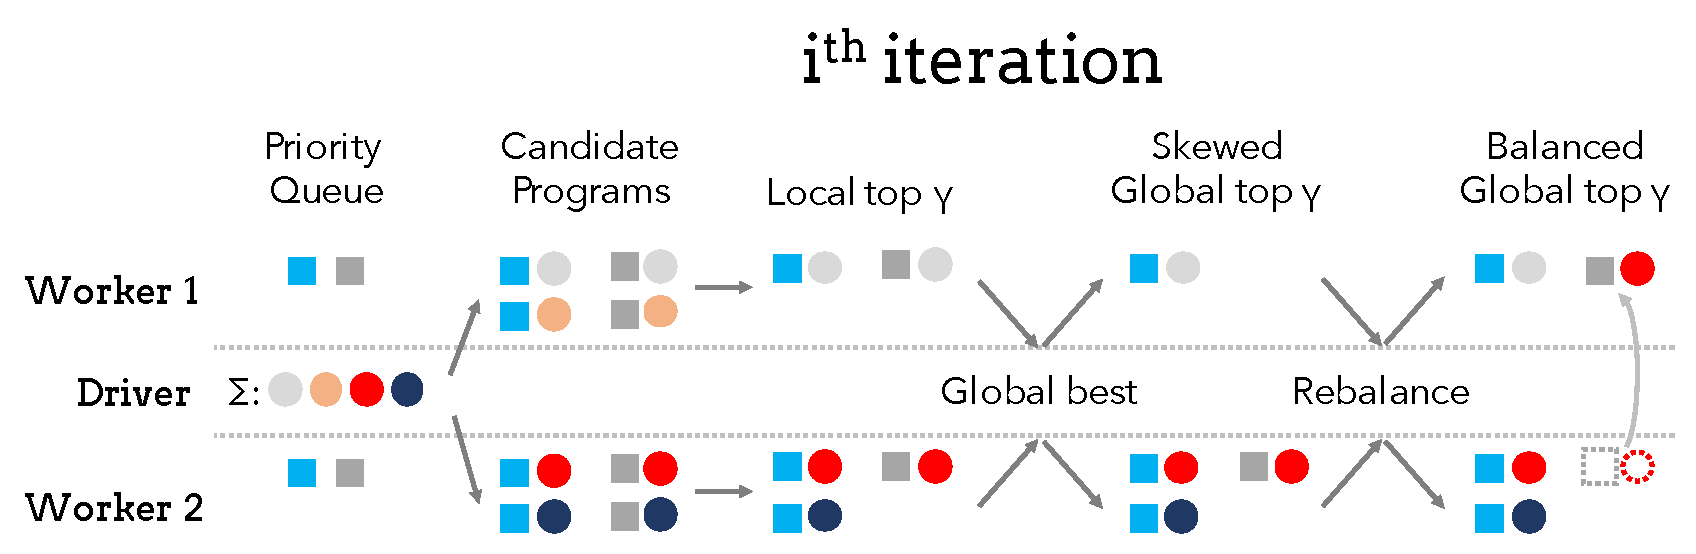
\includegraphics[width=\columnwidth]{figures/distributed.pdf}
    \caption{In each iteration, each worker starts with a subset of the priority queue (boxes).  The driver sends a subset of data transformations from $\Sigma$ (circles) to generate candidate programs (box-circles).  A series of synchronization points identify the globally top $\gamma$ candidates and redistributes them across the workers.   \label{fig:algo}}
\end{figure}

\section{Search Optimizations}\label{s:opts}
This section describes two important optimizations that allows \sys to generate programs efficiently.

\subsection{Parallelization}\label{s:parallel}
Composing and evaluating $Q(p'(R))$ is the single most expensive operation in the search procedure.   We now discuss how we parallelize its evaluation in shared memory and distributed settings, and the challenges when combining it with materialization.

\stitle{Shared Memory} In a naive, shared-memory implementation, we execute all expansions for a given $p\in P$ in parallel.  We materialize $p(R)$ in memory, and evaluate the quality of each $p' = p\circ T\ |\ T \in \Sigma$ in parallel using a  thread pool.  Each thread drops a given $p'$ if its quality is lower than $\gamma\times$ the maximum quality from the previous \texttt{WHILE} iteration or the local thread.  At the end of the \texttt{WHILE} iteration, the threads synchronize to compute the highest quality, and flush the remaining candidates using the up-to-date quality value.  The output of each $p'(R)$ can be retained or discarded using any cache replacement policy.  Our implementation uses Ray~\cite{ray} to schedule and parallelize the tasks.

\stitle{Distributed}
In the distributed setting, we do not have access to fast shared memory and the communication costs of sharing intermediate relations $p(R)$ can be impractical.  Thus, each worker is given a subset of candidate programs to locally evaluate and prune, and the main challenge is to reduce task skew through periodic rebalancing.  We use a worker-driver model with $j$ workers (\Cref{fig:algo}).

Let $P^{next} = P\times \Sigma$ be the set of candidate programs (e.g., 
\includegraphics[height=8pt]{figures/program.pdf}) to evaluate in the current iteration of the search algorithm. For instance, $P=\{NOOP\}$ in the first iteration, so the candidates are the set of individual data transformations $\Sigma$.   The driver assigns the input relation $R$ and $\frac{1}{j}$ of $P^{next}$ to each worker.  In the figure, the driver assigns a subset of $\Sigma$ to each worker.  Each worker evaluates and computes the top-$\gamma$ candidates based on the best worker-local quality.   The worker runs and caches the parents of its assigned candidate programs (
\includegraphics[height=8pt]{figures/sq-blue.pdf}, 
\includegraphics[height=8pt]{figures/sq-grey.pdf}) to incrementally compute the quality function.
  
Note that the worker-local top-$\gamma$ candidates are a superset of the top-$\gamma$ global candidates because the best local quality is $\le$ the global best.   Thus the workers synchronize with the driver to identify the global best candidate and further prune each worker's top candidates.  At this point, all candidate programs are within $\gamma$ of the globally best candidate, but their distribution across the workers can be highly skewed.  \sys performs a final rebalancing step, where each worker sends the number of un-pruned candidates to the driver.  Workers with more than $\frac{1}{j}$ of the total number redistribute the extras to workers with too few candidates.  When redistributing, workers communicate directly and do not involve the driver (e.g., Worker 2 sends 
\includegraphics[height=8pt]{figures/program-greyred.pdf} to Worker 1).   If the total number is $<k$, then candidates are randomly chosen to be replicated.  Only the programs and their qualities are sent; the program results are re-computed by the receiving worker.  This ensures that the priority queue in the next iteration is evenly distributed across all workers.  

% The workers then communicate the quality of their best transformation. This can be used to reconcile the local materializations to only the global top-$\gamma$ set.  This set is not necessarily balanced, e.g., one worker might have almost all of the top transformations.  The next step is a balancing step, where each worker communicates the number of materialized expansions it currently stores.  The workers with more than $\frac{|O|}{j}$ materialized expansions  randomly select ones to evict, and the driver re-distributes these to nodes with too few materialized expansions.  This is done by communicated the transformation and the result is re-computed on the new worker.  If $|O| < k$, then expansions are chosen at random to be replicated.  The result of the reconciliation step is that all workers have an evenly distributed set of materialized expansions.

% \item \ititle{Next Round} After reconciliation, each worker is associated with a particular $o \in O$ (or a set of them). To parallelize, the driver must simply ensure that it assigns new expansions only to those workers that have materialized the parent.  The algorithm then repeats, expanding each node locally, and then reconciles the results.

% The best-first search algorithm also is amenable to parallelization. One can parallelize over the two inner for loops $O \times L$. Each expansion can be forked into its own thread. However, this actually makes the materialization described above a bit more challenging. We use Ray~\footnote{https://github.com/ray-project/ray} to implement the parallel search. 
% 
% \subsubsection{Shared Memory Parallelization}
% The most straight-forward case is when we have access to low-latency shared memory between the expansion threads. In each expansion round, the main thread will assign each expansion node to workers and they will evaluate a given transformation. Each worker will make a copy of $o(R)$ (the node it is expanding) into shared memory. 
% If the expanded transformation is within $\gamma$ of the best current result, then it will update the copy, otherwise delete it. 
% 







\subsection{Dynamically Learning Pruning Rules}\label{s:dynlearn}
To effectively search through the language of transformations, pruning heuristics are important, yet hand-writing such heuristics {\it a priori} is challenging.
We describe how such heuristics can be automatically learned during the search process.


\stitle{Approach}
When \sys executes the search algorithm on each block of data, it generates a program that optimizes the quality metric for that block.  In many cases, the dataset can be partitioned into a large number of blocks that each serve as sources of training examples for a learned pruning model.  Each transformation in a block's  program $p_b$ can be labeled as a positive training example in $\Sigma_b^+$, while all other transformations serve as negative examples $\Sigma_b^- = \Sigma - \Sigma_b^+$.
As \sys processes more blocks, the union of these training sets can be sufficient to train a classifier to predict whether a given transformation will be included in the optimal program.  In our approach, the prediction model $M(T): \Sigma \mapsto \{0,1\}$ is over the data transformations and not the data; is this sense, \sys learns static pruning rules in a dynamic fashion.    

% \sys executes the search on each block of data.  The result is a sequence of transformations to optimize the quality metric on that block.  Every transformation in this sequence can be treated as a positive training example $L^+$, and every transformation not in this sequence can be treated as a negative example $L^-$.  The idea is that if we apply the search to a sufficient number of blocks then we can train a classifier to predict whether a transformation will be included in the final sequence.  It is important to note that this prediction is over the transformations and not the data. 

Internally, \sys uses a Logistic Regression classifier that is biased towards false positives (i.e., keeping a bad search branch) over false negatives (e.g., pruning a good branch). This is done by training the model and shifting the prediction threshold until there are no False Negatives. 


\stitle{Featurization}
To use this approach, we use featurizers to transform each data transformation $T$ into a $k$-dimensional feature vector: \textsf{feat}: $T\mapsto\mathbb{R}^k$.
For example, recall the \texttt{find\_replace(NYC, NY, city\_code)} transformation in~\Cref{ex1}.
The expert is free to encode potential signals as part of the transformation.  For instance, the edit distance between the two literal parameters (e.g., NYC, NY) and an indicator vector to specify the attrbitue (e.g., city\_code).  

Notice that many data transformation can be modeled as a predicate that specifies which records to clean, target attributes to clean, and replacement values for those attributes.  Thus, the featurized transformation potentially allows a model to learn which records, which attributes, and what replacement values, are highly to contribute to the final program.  For instance, \sys may learn that \texttt{find\_replace} only makes sense for \texttt{city\_name}.  Similarly, it may learn that the replacement string should be similar in edit distance to the source string, and subsequently learn the appropriate edit distance threshould.


\stitle{Discussion} We believe this is one of the reasons why a simple best-first search strategy can be effective.  For the initial blocks, \sys searches without a learned pruning rule in order to gather evidence.  Over time, the classifier can identify systematic patterns that are unlikely to lead to the final program, and explore the rest of the space.  In fact, this incremental learning process can be viewed from an active learning perspective to further target the exploration towards programs that will best improve the classification model.  
A potential benefit of learning a pruning model for {\it data transformations} rather than relation instances is that it can potentially be reused or fine-tuned for new, but structurally similar, data transformation problems. In this way, the model can be trained {\it across data transformation problems} rather than across blocks within a single problem.    


% For example, some columns might not be dirty and are not worthwile to clean.  In the example above, another observation could be that the source and target strings in the optimal sequence are very close in terms of string similarity (as opposed to arbitrary transformations).  If each of these operations was featurized with a single scalar that is the edit-distance between the two strings, then the classifier could learn a pruning threshold (i.e., not considering find-and-replace operations above that threshold).  

% Consider an alternative to a predefined search heuristic where we clean data in small blocks.  For the initial blocks, we search without a heuristic.  As we continuously perform the search, we train a classifier on these features to reject search branches that are not typically in the final solution.  This allows us to exploit any patterns in the literal parameters that repeatedly occur.




%Notes

% * Exp 1. Precision and recall: detection of inverse transformations

% * Exp 2. Efficiency in special cases

% * Exp 3. Case Studies
%Existing datasets

\section{Experiments}\label{s:exp}
To the best of our knowledge a comparable explanation system to \sys does not exist, so we evaluate \sys in a comprehensive study against reasonable baselines. This meant piecing together data cleaning and outlier detection systems into pipelines (sometimes combining them with learning) to illustrate the benefits of \sys.  

\subsection{Synthetic Data}
In the first set of experiments, we characterize \sys on synthetic data. We generate a dataset with the following schema:
\begin{lstlisting}
City(Name, Abreviation, Population)
\end{lstlisting}
Names are randomly generated from a set of strings scraped from wikipedia, abbreviations are generated from two letters randomly selected from the names, and populations are generated via a Zipfian distribution. This dataset considers multiplicities where there are duplicate (non-erroneous) records.

\stitle{Anomalies}
We consider a number of different anomaly detection criteria:
\begin{itemize}[leftmargin=*, topsep=0mm, itemsep=0mm]
    \item \textbf{Q1: } All records that violate a one-to-one mapping constraint between \texttt{Name} and \texttt{Abbrevation}. This is a standard functional dependency constraint to detect anomalies~\cite{DBLP:conf/sigmod/ChalamallaIOP14}.
    \item \textbf{Q2: } All records with a population greater than 6 median absolute deviations from the median population. This is a standard quantitative outlier detection condition to detect anomalies~\cite{bailis2016macrobase,scorpion}. 
    \item \textbf{Q3: } All records whose abbreviation has a string length not equal to two. This is a more complex UDF that cannot be addressed by existing work.
\end{itemize}
For each of these anomaly detection criteria, we generate errors in the dataset. For Q1, we select a random subset of each of the records with a particular name and perturb the \texttt{Abbrevation} attribute. For Q2, we randomly generate populations with a population of 0 or one that is much higher than typical and replace a subset of records that satisfy a equality predicate on either \texttt{Name} and \texttt{Abbrevation} or both.
For Q3, we randomly add characters to some records abbrevations.

\stitle{Language}
We consider different parametrized languages for transformations:
\begin{itemize}[leftmargin=*, topsep=0mm, itemsep=0mm]

    \item \textbf{D1: } All deletions with a single attribute equality predicate.

    \item \textbf{D: } All deletions with a multiple attribute equality predicate. This setting of \sys is the most similar to prior outlier explanation work.

    \item \textbf{R1: } All single attribute find and replace operations.

    \item \textbf{R: } All multiple attribute find and replace operations. This setting of \sys is most similar to prior data cleaning work.

    \item \textbf{M: } All transformations on the population attribute that clip all values above or below a discretized threshold.
\end{itemize}

\subsubsection{Absolute Runtime and Accuracy}
Due to the way that we generated errors, we have a natural notion of ground truth. We know the predicates and transformations used the generate errors, and we can calculate the precision and recall. For a generated dataset of 10000 records, we tuned the error generation process such that approximately 5\% of records are corrupted. The tables (Table \ref{t1} and Table \ref{t2}) show the F1 score of \sys for all combinations of languages and detectors and the runtimes for each of the pairs in seconds. 
We use `*' to indicate combinations that are comparable with prior explanation and cleaning systems. 

\sys provides flexibility to the user the change the language and the quality functions to elict different behaviors. For example, the R and R1 languages are not suited for numerical manipulation. The M language can be used to improve accuracy. The runtime of \sys largely depends on how large the support of the language is. More carefuly designed languages lead to faster and more accurate transformation programs. More complex quality functions only impact runtime in terms of how expensive they are to compute.

\begin{table}[t]
\centering
\begin{tabular}{
>{\columncolor[HTML]{000000}}l llll}
{\color[HTML]{FFFFFF} }   & \cellcolor[HTML]{000000}{\color[HTML]{FFFFFF} Q1} & \cellcolor[HTML]{000000}{\color[HTML]{FFFFFF} Q2} & \cellcolor[HTML]{000000}{\color[HTML]{FFFFFF} Q3} & \cellcolor[HTML]{000000}{\color[HTML]{FFFFFF} Q123} \\
{\color[HTML]{FFFFFF} D1} & 1.0                                               & 0.89                                              & 1.0                                               & .88                                                 \\
{\color[HTML]{FFFFFF} D}  & 0.84                                              & .86*                                              & 1.0                                               & .79                                                 \\
{\color[HTML]{FFFFFF} R1} & 1.0                                              & {\color[HTML]{000000} .71}                        & 1.0                                               & .86                                                 \\
{\color[HTML]{FFFFFF} R}  & 0.83*                                              & .68                                               & 1.0                                               & .77                                                 \\
{\color[HTML]{FFFFFF} M}  & -                                                 & 1.0                                               & -                                                 & -                                                  
\end{tabular}
\caption{The F1 score of \sys for all languages and detector combinations. The starred entries are settings of \sys for which a comparable system exists.}
\label{t1}
\end{table}


\begin{table}[t]
\centering
\vspace{.2in}
\begin{tabular}{
>{\columncolor[HTML]{000000}}l llll}
{\color[HTML]{FFFFFF} }   & \cellcolor[HTML]{000000}{\color[HTML]{FFFFFF} Q1} & \cellcolor[HTML]{000000}{\color[HTML]{FFFFFF} Q2} & \cellcolor[HTML]{000000}{\color[HTML]{FFFFFF} Q3} & \cellcolor[HTML]{000000}{\color[HTML]{FFFFFF} Q123} \\
{\color[HTML]{FFFFFF} D1} & 8.1                                               & 3.5                                               & 5.4                                               & 12.9                                                \\
{\color[HTML]{FFFFFF} D}  & 32.9                                              & 24.1*                                              & 21.9                                              & 59.3                                                \\
{\color[HTML]{FFFFFF} R1} & 17.5                                              & {\color[HTML]{000000} 16.5}                       & 17.8                                              & 25.7                                                \\
{\color[HTML]{FFFFFF} R}  & 107.8*                                             & 59.4                                              & 69.3                                              & 136.9                                               \\
{\color[HTML]{FFFFFF} M}  & -                                                 & 0.17                                              & -                                                 & -                                                  
\end{tabular}
\caption{The runtime of \sys for all languages and detector combinations. The starred entries are settings of \sys for which a comparable system exists.}
\label{t2}
\end{table}

\begin{figure*}
    \centering
    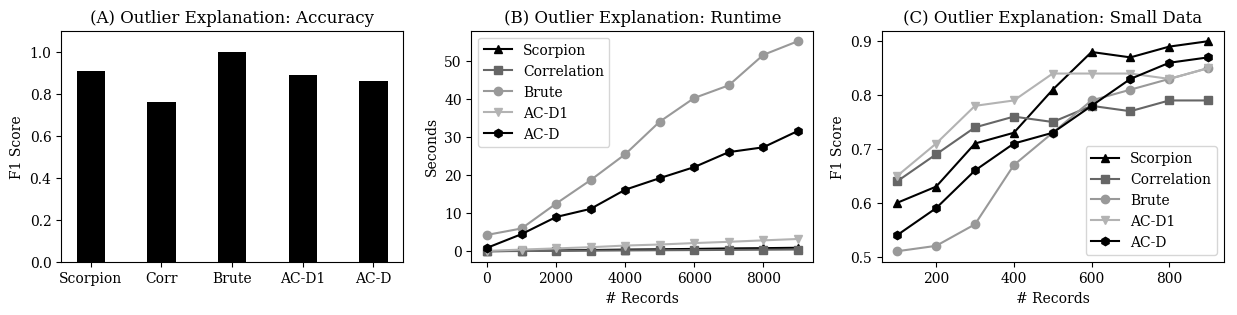
\includegraphics[width=0.8\textwidth]{exp/exp1-new.png}
    \caption{\small Comparison with outlier explanation systems. While, \sys is more general, it is also competitive in terms of accuracy. \label{exp1-new}}
\end{figure*}

\begin{figure*}
    \centering
    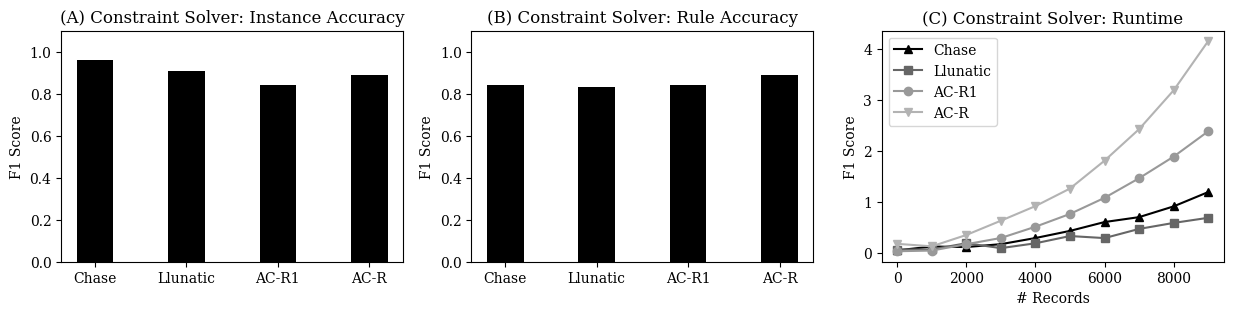
\includegraphics[width=0.8\textwidth]{exp/exp2-new.png}
    \caption{\small Comparison with FD repair systems. As with the outlier explanations, \sys is more general, it is also competitive in terms of accuracy.\label{exp2-new}}
\end{figure*}

\subsubsection{Comparison to Specialized Systems}
Next, we compare \sys to specialized systems where applicable.  First, we compare \sys to outlier explanation algorithms when the quality function is Q2 (numerical outliers) and the language is only deletions (D1, D). We consider the following alternatives: Scorpion~\cite{scorpion} using a decision tree to extract the predicate, correlation that identifies predicates most correlated with the outliers inspired by and avoids evaluating all subsets of attributes~\cite{bailis2016macrobase}, brute force which enumerates all predicates and returns the one with the highest correlation, \sys with a single attribute predicate (AC-D), and \sys with a multiple attribute predicate (AC). Figure \ref{exp1-new} plots the results for F1 score on 10000 records, runtime, and the F1 score as a function of number of records.
\sys is competitive in terms of accuracy in the specialized cases, but is more expensive in terms of runtime.
The run time of \sys can be improved by changing the language specification (e.g., restricting the search to a single attribute deletion).

Another intriguing result is the accuracy on a small dataset.
Since the alternatives, Scorpion and Brute Force, search over multiple attributes by default. They are susceptible to overfitting to spurious trends when the dataset is small.
\sys with a single attribute predicate actually achieves an improved accuracy result for a smaller dataset.
The flexibility in language can be used as a form of regularization to avoid overfitting.

Next, there is overlap between \sys and data cleaning systems. We next compare to standard functional dependency enforcement algorithms on the quality function Q1 (one-to-one relationship) and the replacement langugages (R1 and R). We compare \sys to a restricted chase algorithm~\cite{benedikt2017benchmarking} and a tuple-generating dependency-based cleaning system called Llunatic~\cite{DBLP:conf/sigmod/DallachiesaEEEIOT13}. The challenge is that these systems do not return rules but return cleaned instances of the database. So, we extract rules from the edits using a decision tree as in scorpion. Then, we compare the systems on two different accuracy metrics: instance accuracy (how well do the transformations recover the true values), and rule accuracy (can we explain the edits with rules). 

Figure \ref{exp2-new} illustrates the results. While \sys is slower than the specialized constraint enforcement systems in terms of runtime, it is competitive in terms of accuracy--especially when it comes to extracting transformation rules. The constraint solving systems operate at a tuple-by-tuple basis and do not necessarily ground their solutions in predicates.

\subsection{Real Case Studies}
Beyond the characterization, we consider 7 case studies applying \sys to real problems. When relevant, we present ``best effort'' comparisons with existing systems--as in the synthetic experiments.

\stitle{Flight} The flight dataset~\cite{data-flights} contains arrival time, departure time, and gate information aggregated from 3 airline websites (AA, UA, Continental), 8 airport websites (e.g., SFO, DEN), and 27 third-party websites.
There are 1200 flight departures and arrivals at airline hubs recorded from each source.  Each flight has a unique and globally consistent ID, and the task is to reconcile data from different sources using the functional dependency \texttt{ID$\rightarrow$ arrival, departure, gate information}.

\stitle{FEC} The election contributions dataset has 6,410,678 records, and 18 numerical, discrete, and text attributes. This dataset records the contribution amount and contributor demographic information e.g., name, address, and occupation.  The task is to enforce \texttt{city$\rightarrow$zipcode}, and match occupation to a codebook on canonical occupations.  The quality function is 1 if the occupation is in the codebook, and 0 otherwise; we penalize the edit distance between the original and edited occupation values.

\stitle{Malasakit} This dataset contains 1493 survey disaster preparedness responses from the Philippines, with 15 numeric and discrete attributes. The task removes improper numerical values and remove dummy test records. This consists of domain integrity constraints that force the values to be within a certain dictionary.

\stitle{Physician} This dataset from Medicare.gov contains 37k US physican records, 10 attributes, with spelling errors in city names, zipcodes, and other text attributes. We use the rules described in~\cite{rekatsinas2017holoclean}, which consists of 9 functional dependencies for error detection. 

\stitle{Census} This US adult census data contains 32k records, and 15 numeric and discrete attributes.  There are many missing values coded as 999999.  The task is to clean numeric values to build a classification model that predicts whether an adult earns more than $\$50k$ annually. 

\stitle{EEG}  The 2406 records are each a variable-length time-series of EEG readings (16 numeric attributes), and labeled as ``Preictal'' for pre-seizure and ``Interictal'' for non-seizure.  The goal is to predict seizures based on 32 features computed as the mean and avriance of the numeric EEG attributes.  The task is to identify and remove outlier reading values.  

\stitle{Terrorism} The Global Terrorism Database~\cite{data-terrorism} is a dataset of around terrorist attacks scraped from news sources.  Each record contains the date, location, details about the attack, and the number of fatalities and injuries.  The dataset contains a mixture of data errors:
(1) there are many duplicates for the same terrorist incident,
(2) many missing values in the fatalities and injuries attributes are encoded as zeros, which overlaps with attacks that did not have any fatalities/injuries, and
(3) the location attributes are inconsistently encoded.  
We used the dataset from 1970, and there are $170000$ records.  
We downloaded this dataset and sought to understand whether terrorist attacks have become more lethal than they were in the 1970s.  To do so, we hand cleaned the records to create a gold standard.  It turns out that, in this dataset, attacks have become more lethal, but fewer in number than 50 years ago.  This task was intentionally open-ended to represent the nature of the iterative analysis process.


\begin{figure}
    \centering
    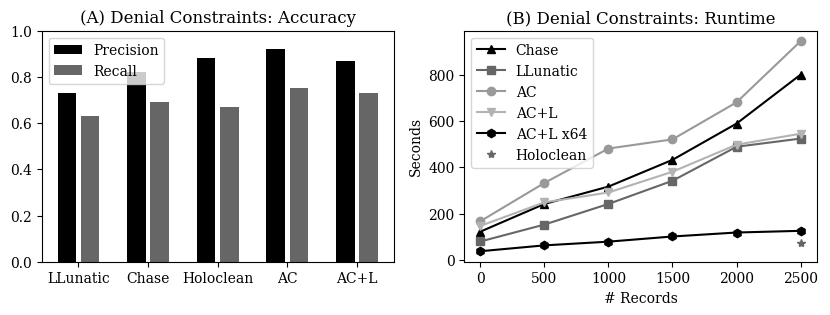
\includegraphics[width=\columnwidth]{exp/exp1.png}
    \caption{\small Comparison with denial constraint systems on the Flight dataset.  (A) \sys (AC) matches or exceeds the accuracy of the specialized systems.  (B) The structure of the data errors, along the learning and parallelization (AC+L x64) lets \sys scale sub-linearly and outperform all but HoloClean's reported runtimes.  \label{exp1a}}
\end{figure}

\subsection{Detecting Anomalies with Constraints}
In the first set of case studies, we consider the Flight, Physician, FEC, and Malasakit datasets. In these datasets, the errors can be effectively detected as denial constraints. Denial constraints express a wide range of integrity constraints and form the basis of many data cleaning systems.  One can imagine a user interactively generating these constraints and observing what types of transformations are generated to enforce the constraints. We can compose a quality function that quantifies the number of constraint violations and find transformations that reduce the number of violations. For \sys, we search over single attribute find and replace transformations (R1 in the synthetic experiments). We quantify the precision and recall of the transformations discovered. 

\stitle{Baselines}  We tried to piece together explanation pipelines using existing data cleaning software, i.e., generate a cleaned instance for each constraint and then infer rules from those instances (as in the synthetic experiment). We compare \sys on instance-level accuracy to gold standard ground truth cleaned by hand. We run against (1) Llunatic, a denial constraint-based cleaning system~\cite{DBLP:conf/sigmod/DallachiesaEEEIOT13} implemented in C++ on top of PostgreSQL\footnote{Constraints are specified as Tuple-Generating Dependencies}, and (2) a restricted chase algorithm~\cite{benedikt2017benchmarking} implemented in Python. We compare against the chase because a large portion of denial constraints are functional dependencies, and can be resolved using fixed-point iteration.  We report numbers from the recent Holoclean publication~\cite{rekatsinas2017holoclean} that used the same datasets and constraints, but did not run the experiment ourselves.

\stitle{Results} Figure \ref{exp1a}a shows the precision and recall of each approaches based on known ground truth. \sys matches or beats the accuracy of the baselines, however its runtime (AC) without any learning scales poorly compared to alternatives (Figure~ \ref{exp1a}b).  Using learning (AC+L) shows performance on par with LLunatic, and parallelization on 64 threads is comparable to Holoclean's reported runtime. The results suggest that learning exhibits sublinear scaling due to \sys learning more effective pruning rules as it sees more data.  These performance gains are at the expense of slightly reduced accuracy. 

There are both positives and negatives in these results. \sys is slow compared to the specialized solutions but greatly reduces the engineering complexity of having to design them and compose them with a rule extraction interface. More research is needed into this class of algorithms in the future to reduce the runtime gap.

We also evaluated \sys (single threaded, without learning) on the FEC, Malasakit, and Physician datasets.  Their precision, recall, and runtimes are as follows: 
FEC: $94\%$ prec, $68\%$ rec; 
Malasakit: $100\%$ prec, $85\%$ rec;
Physician: $100\%$ prec, $84\%$.

\begin{figure}
    \centering
    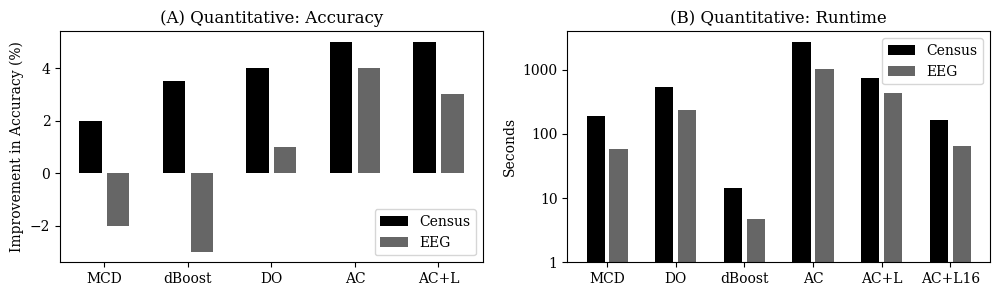
\includegraphics[width=\columnwidth]{exp/exp2.png}
    \caption{\small Numerical Transformations on census and EEG datasets for a classification application.  \sys tranformation can clip outliers or set them to a default value. (A) \sys has a higher accuracy than outlier detection algorithms (MCD, dBoost), and \sys with a single transform template (DO).  (B) Optimizations improve \sys runtime by over an order of magnitude.  \label{exp2a}}
\end{figure}

\subsection{Detecting Anomalies with Models}\label{s:expquant}
This experiment performs numerical transformations on machine learning data.  We explore to what extent the transformations provided by \sys can be used to improve the performance of a downstream data product such as machine learning. In these applications, prediction labels and test records are typically clean and available (e.g., results of a sales lead), whereas the training features are often integrated from disparate sources and exhibit considerable noise (e.g., outliers).  Our quality function is simply defined as the model's accuracy on a training hold-out set, and we report the test accuracy on a separate test set.

We trained a binary classification random forest model using \texttt{sklearn} on the Census and EEG datasets.  We used standard featurizers (hot-one encoding for categorical data, bag-of-words for string data, numerical data as is) similar to~\cite{gokhale2014corleone}. 
We split the dataset into 20\% test and 80\% training, and further split training into 20/80 into hold-out and training.  We run the search over the training data, and evaluate the quality function using the hold-out.  Final numbers are reported using the test data.

We defined the following three data transformation templates that sets numerical attribute values in $R$ if they satsify a predicate:

{\small
\begin{itemize}[leftmargin=*, topsep=0mm, itemsep=0mm]
  \item \stitle{\textsf{clip\_gt(attr, thresh)}} $R.attr = thresh$ if $R.attr>thresh$
  \item \stitle{\textsf{clip\_lt(attr, thresh)}} $R.attr = thresh$ if $R.attr<thresh$
  \item \stitle{\textsf{default(attr, badval)}} $R.attr$ set to mean val if $R.attr=badval$
\end{itemize}
}

\stitle{Baselines} As before, we constructed best effort pipelines with existing tools. Composing outlier detection software with reasonable default transformations. These tools leverage the data to identify outliers, while \sys leverages the quality function (i.e., the model's own confidence metric).
We compare with 4 baselines: {\it No Transformation (NC)}, {\it Minimum Covariance Determinant (MCD)} is a robust outlier detection algorithm used in~\cite{bailis2016macrobase} and sets all detected outliers to the mean value, {\it dBoost} uses a fast partitioned histogram technique to detect outliers~\cite{mariet2016outlier}, and {\it Default Only (DO)} runs \sys with only the \textsf{default()} transformation.  

\stitle{Results} The classifer achieves 82\% and 79\% accuracy on the uncleaned census and EEG data, respectively.  Most outliers in the census data are far from the mean, so MCD and dBoost can effectively find.  Further, setting census outliers to the mean is sensible. However, the same fix is not appropriate for the EEG data; it is better to clip the outlier values, thus MCD, dBoost, and DO have negligible or negative impact on accuracy.  When we realized this from running DO, it was straightforward to add the clipping transformations to the language, and with no other changes, re-run \sys with drastically improved EEG accuracies.  
Vanilla \sys (AC) is nearly $10\times$ slower than MCD, but the adding learning and 16-thread parallelization  matches MCD's runtimes.  dBoost is specialized for fast outlier detection and \sys is unlikely to match its runtime.  


\begin{figure}[ht]
    \centering
    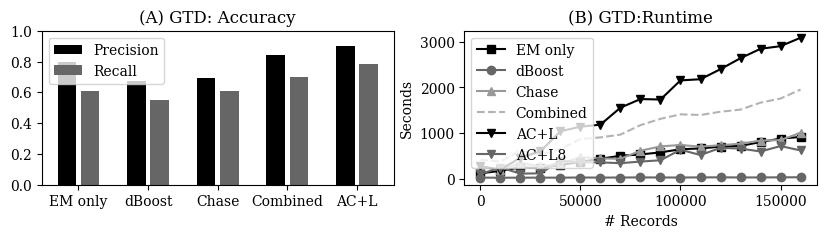
\includegraphics[width=\columnwidth]{exp/exp7.png}
    \caption{The Global Terrorism Database is a dataset of terrorist attacks scraped from news sources since 1970. (A) Shows that \sys can integrate many different forms of transformations that were previously handled by disparate systems, (B) \sys achieves a competitive runtime to using all of the different system and accounting for data transfer time between them. \label{exp7a}}
\end{figure}

\subsection{Mixing Error Classes}\label{s:expterror}
The power of \sys is seen in datasets where there are multiple types of anomalies.
We use the multi-error Terrorism dataset as such an example ~\cite{data-terrorism}. 

\stitle{Baselines} We constructed a pipeline consisting of a hand-coded blocking-based entity matching (EM), a restricted chase (FD) algorithm in Python, and used dBoost for missing values.  We ran EM, dBoost, and Chase serially on the dataset (Combined). We use that combination to generate transformation explanations.
This is compared to \sys where there is one framework with different quality functions. We use a library of transformation consisting of find-and-replace operations as well as the numerical transformations described previously.


\stitle{Results} \Cref{exp7a}a shows that combining  all three classes of errors within the same \sys framework (AC) achieves higher precision and recall than all baselines.  In fact, the combined baselines still does not achieve \sys's level of accuracy because the  operations need to be interleaved differently for different blocks.   Although \sys is slower than any individual baseline, parallelizing \sys to 8 threads is faster than the combined baseline by 2x. 


 \begin{figure*}[t]
\centering
 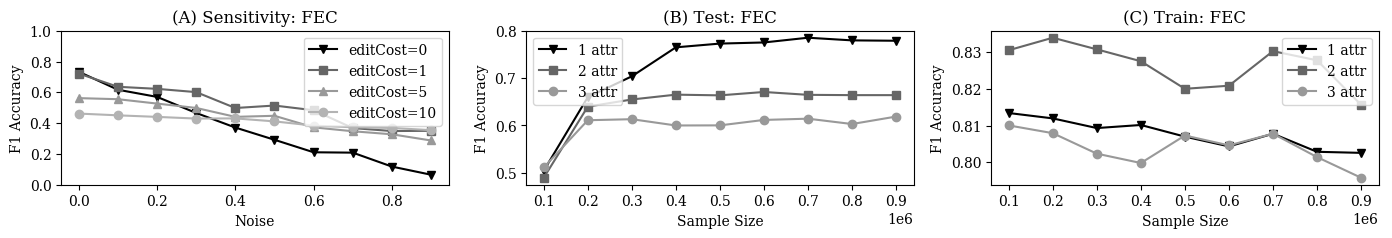
\includegraphics[width=\textwidth]{exp/exp5.png}
 \caption{\small (A) Regularization by increasing an editCost penalty makes \sys more robust to noisy (mis-specified) quality functions, (B-C) overly expressive transformation templates can lead to overfitting (2 attr) or an infeasibly large search space (3 attr).  
 \label{fig:sensitivity}}
\end{figure*}

 \begin{figure*}[t]
\centering
 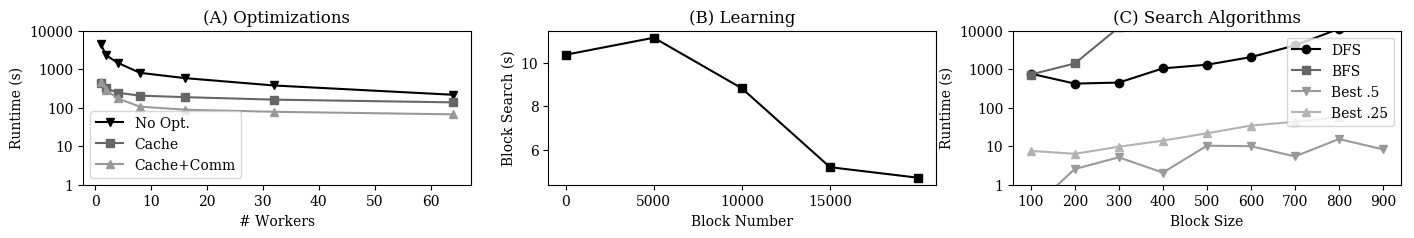
\includegraphics[width=\textwidth]{exp/exp6.png}
 \caption{\small 
   (A) Both the materialization (Cache) and distributed communication (Comm) optimizations contribute to improved scale-out runtimes.
   (B) The learned pruning rules improve the search costs for each subsequent block-wise partition.  
   (C) Best-first search is better than BFS and DFS; reducing $\gamma$ prunes more candidates at the expense of lower accuracy.  
 \label{fig:opt}}
\end{figure*}

\subsection{\sys In Depth}
This subsection uses the FEC setup to study the parameters that affect \sys's accuracy and runtime, the robustness of its transformation programs, and its algorithmic properties.

\subsubsection{Algorithmic Sensitivity}

\stitle{Partitioning} Partitioning the dataset into smaller blocks effectively reduces the problem complexity.  This can have tremendous performance benefits when each block exhibits very few errors that are independent of the other blocks.  \Cref{fig:microbenchmarks}a shows the performance benefits when varying the block size; we define the blocks by partitioning on three different attributes that have different domain sizes.  Reducing the block size directly improves the runtime; the search is effectively non-terminating when blocking is not used.    

\stitle{Language} \Cref{fig:microbenchmarks}b fixes the input to a single block, and evaluates the runtime based on the size of the language $|\Sigma|$.  Increasing the transformations increases the branching factor of the search problem. The search time is exponential in the language, however \sys's learning optimization can identify a pruning model that reduces the runtime to linear.

\stitle{Coupling in the Quality Function} The complexity of the quality function directly affects search time.  A cell-separable quality function is the simplest to optimize because each cell in the relation can be analyzed and cleaned in isolation.  In contrast, a quality function that couples multiple records together is more challenging to optimize because a longer sequence of transformation may be needed to sufficiently clean the records and improve the quality function.  

We evaluate this by artificially coupling between 1-10 records together, and creating a quality function that only improves when an attribute of the coupled records all have the same value.  We perform this coupling in two ways: {\it Random} couples randomly selected records, whereas {\it Correlated} first sorts the relation an attribute and couple records within a continuous range.  We expect that the random coupling requires individual operations for each record based on their IDs, whereas the correlated setting both allows \sys to exploit the correlated structure to learn effective pruning rules and to clean the coupled records using a single operation.  \Cref{fig:microbenchmarks}c shows that this is indeed the case when running \sys on a single fixed-size block. {\it Random} slows down exponentially with increased coupling, whereas {\it Correlated} increases linearly.

% The nature of the quality function also affects the search time. Quality functions that couple multiple records together are harder to optimize (Figure \ref{fig:microbenchmarks}c).
% Consider a function that requires that two different records must have the same attribute values.
% More transformations have to be achieved in a particular sequence before an improvement in quality is observed. 
% We selected between 1-10 records at random in each block and created a quality function that coupled these records together.
% As the degree of coupling increases, the search time grows quite drastically.
% We repeated the same experiment where now coupling is correlated with the data, i.e., we sort one of the attributes and couple ``nearby'' records.
% \sys performs significantly better on this version of the task.
% This is due to the learned pruning in \sys.
% Sorting the attributes introduces a systematic correlation in the quality function.
% \sys quickly learns a model which learns this correlation and uses that to prune the search space.

\stitle{Quality Function Complexity} Finally, we incrementally increase the quality function's complexity and show haw it affects the accuracy.  We add the following constraints in sequence: one functional dependency (FD), a second FD, an entity resolution similarity rule, and a third FD.  We define the quality function as the sum of each constraint's quality function.   \Cref{fig:microbenchmarks}d shows that the F1 accuracy decreases as more constraints are added, however the F1 score is still above $75\%$.  


\subsubsection{Generalization and Overfitting}\label{s:expoverfit}
An important characteristic of generating transformation solutions as {\it programs} is that we can evaluate the program's robustness in terms of machine learning concepts such as overfitting and generalization.    To this end, we examine two concepts in the context of data transformations: regularizaton and overfitting.  We also find that \sys's high level interface is helpful for iteratively tuning the transformation process.

\stitle{Regularization}  Misspecified quality functions can cause \sys to output poorly performing transformation programs.  We simulate this by adding random noise to the output of the quality function. \Cref{fig:sensitivity}A plots the F1-score of \sys on the FEC experiment while varying the amount of noise.  As expected, the output program's F1-score rapidly degrades as the noise increases.  

Machine learning uses regularizing penalty terms to prevent overfitting.  We can similarly add a penalty to the quality function to prevent too many edits.  Each line line shows the edit cost penalty and shows that although the F1 is lower when there is no noise, \sys is more robust to larger amounts of noise. 

\stitle{Overfitting} In machine learning, over-parameterized models may be susceptible to overfitting.  A similar property is possible if the language $\Sigma$ is overly expressive.  We use a transformation template that finds records matching a parameterized predicate and sets an attribute to another value in its instance domain.   We then vary the language expressiveness by increasing number of attributes in the predicate between 1 and 3.  Finally, we run \sys on a training sample of the dataset (x-axis), and report F1 accuracy on the training and a separate test sample (\Cref{fig:sensitivity}B-C).  Note that overfitting occurs when the training accuracy is significantly higher than test accuracy.

Indeed we find an interesting trade-off.  The 1 attribute predicate performed worst on the training sample but outperformed the alternatives on the test sample.  The 2 attribute predicate was more expressive and overfit to the training data.  Finally, the 3 attribute predicate is overly expressive and computationally difficult to search.  Thus, it did not sufficiently explore the search space to reliably identify high quality transformation programs. 

\stitle{Discussion} We have shown that data transformations can overfit, and believe this is a potential issue in {\it any} transformation procedure. These results highlight the importance of domain experts to judge and constrain the problem in ways that will likely generalize to future data. Further, it shows the value of a high-level interface that experts can use to express these contraints by iteratively tuning the quality function and transformation language. 

% and evaluate the training and test        Figure \ref{fig:sensitivity}B-C illustrates another interesting aspect of \sys, namely, a property akin to overfitting in machine learning.
% We parametrized the transformation language with single attribute, double attribute, and triple attribute predicates.
% Then, we applied \sys to sample of data.
% We measured the ``in-sample error'' Figure \ref{fig:sensitivity}C, which is the F1 score with records inside the sample, and the ``out-of-sample'' error which is the F1 score on unseen records.
% The more expressive two attribute predicates are most accurate on the in-sample metric, however, we not as accurate as the single attribute predicates on the out-of-sample metric.
% The three sample predicates were very computationally expensive to search so the results are less reliable.
% This result highlights an important point overly specific rules may not apply to future data, and overly general rules, might introduce unwanted side-effects.


\subsubsection{Scaling}
Next, we present preliminary results illustrating the scaling properties of \sys. 

\vspace{1em}

\stitle{Parallelization Optimizations} The experiments run on a cluster of 4 mx.large EC2 instances, and we treat each worker in a distributed (not shared-memory) fashion.   \Cref{fig:opt}a shows the benefits of the materialization and communication optimizations in \Cref{s:parallel}.  {\it No opt.} simply runs best-first search in parallel without any materialization; workers only synchronize at the end of an iteration by sending their top-$\gamma$ candidate programs to the driver, which prunes and redistributes the candidates in the next iteration.  {\it Cache} extends No opt by locally materializing parent programs, and {\it Cache+Comm} further adds the communication optimizations for distributed parallelization.   

The single threaded No Opt setting runs in $4432$s, and the materialization optimization reduces the runtime by $10\times$ to $432$s.   Scaling out improves all methods: at 64 workers, {\it Cache+Comm} takes 67s while {\it Cache} takes 137s.  Surprisingly, although {\it No Opt} with 64 workers is slower than {\it Cache+Comm} by $10\times$, it scales the best because it only synchronizes at the end of an iteration and only communicates candidate programs and their quality values.  In contrast, the alternative methods may communicate materialized relation instances.  

\stitle{Within-Block Learning} Although we have shown how learning reduce the overall search runtime, we show that learning also improves the search speed for individual blocks.  We run single-threaded \sys and report the time to evaluate each block.  \Cref{fig:opt}b shows the $i^{th}$ block that is processed on the x-axis, and the time to process it on the y-axis.   We see that as more blocks are cleaned, the learned pruning classifier is more effective at pruning implausible candidate programs.  This reduces the per-block search time by up to $75\%$.  

\stitle{Search Algorithm Choice} \Cref{fig:opt}c shows that best-first search out-performs naive depth and breadth first search.  We also report \sys when $\gamma=\{0.5, 0.25\}$.  We see that as the block size increases, DFS and BFS quickly become infeasible, whereas \sys runs orders of magnitude more quickly.  In addition, reducing $\gamma$ improves the runtime, however can come at the cost of reduced accuracy by pruning locally sub-optimal but globally optimal candidate programs.  



\subsubsection{Program Structure}
Finally, we present results describing the structure of the data transformation programs found with \sys.
It is often the case that the program found by \sys is a concise description of the needed data transformation operations, that is, the total number of cell edits is much larger than the length of the program.
We consider the FEC dataset, the EEG dataset, and GTD dataset.

Sometimes, the program (FEC and GTD) encodes a significant amount of literal values. This happens in entity matching type problems. For these problems, the program length is relatively large, however, the number of cells modified is even larger (up to 10x more).
For datasets like the EEG dataset, the program is very concise (26x smaller than the number of cells modified).
Numerical thresholds are generalize better than categorical find-and-replace operations.

\begin{table}[ht!]
\centering
\label{my-label}
\begin{tabular}{|l|l|l|}
\hline
    & Program Length & Cells Modified \\ \hline \hline
FEC & 6416           & 78342          \\ \hline
EEG & 6              & 161            \\ \hline
GTD & 1014           & 104992 \\ \hline
\end{tabular}
\end{table}


\section{Conclusion and Future Work}
In summary, \sys poses explanation generation as a planning problem over a language of data transformations, and presents existing error-specific approaches---constraint-based, statistical, and demonstration-based data cleaning---within a single framework.
Our results suggest that borrowing from recent advances in planning and optimization is a fruitful direction.  
While we focus on explanation in this work, we are excited to extend \sys towards data cleaning system.  In particular, data cleaning is inherently a visual and interactive process, and we plan to integrate \sys with a data visualization interface.   Users can visually manipulate and examine their dataset and the system can translate interactive manipulations into quality functions.  This will also require work to characterize failure modes and provide high level tools to debug such cases.  We are also hopeful that the compact codebase (<200 LOC for the core search and learning algorithms) can enable more rapid development of specialized data cleaning systems for novel domains and error conditions.  



% The prevailing wisdom in the design of data cleaning algorithms is to exploit the details of specific problem rather than considering the most general cases, and our experiments suggest that this a general framework like \sys can achieve parity in terms of accuracy.
% While the serial implementation of \sys can be much slower than the competitor specialized frameworks, \sys can be efficiently distributed to significantly reduce the gap.
% 
% These results should be considered a proof-of-concept that such a data cleaning \sys can be built around the recent results in AI. 
% However, to us, these results are still counter-intuitive, and raise a number of speculative questions for the future: (1) are specialized systems overly engineered for worst-case guarantees and perhaps real-datasets are not that pathalogical, (2) maybe the benchmarks that we consider in data cleaning are too easy to brute-force, (3) what are the failure modes and corner cases of \sys in real data.
% We hope to consider these problems in future work, as well as extending the system to novel settings.
% In particular, we are interested in \sys as a middleware layer for data visualization.
% A user can manipulate data in a visual UI and these manipulations can be translated into a quality function.
% 

%NSF 1527765, 1564049.
Jiannan







%\bibliographystyle{abbrv}

{
%\fontsize{8.8pt}{9.7pt} \selectfont
\small
\bibliographystyle{abbrv}
\bibliography{ref} 
\scriptsize
}


%\appendix
\label{s:appendix}

\section{Quality Functions}
Details about quality functions for exsiting stuff

\section{Data Transformations}

Details about data xforms that we used.

\section{Datasets}
\vspace{0.5em}\noindent\textbf{USCensus: } This dataset contains US Census records for adults and the goal is to predict  whether the adult earns more than $50,000$ dollars. It contains 32,561 records with 15 numerical and categorical attributes. This dataset contained missing values and coding inconsistencies.
Examples of data error include:
\begin{lstlisting}
#missing values
40,Private,121772,Assoc-voc,11,
Married-civ-spouse,Craft-repair,Husband, 
Asian-Pac-Islander,Male,0,0,40,(*\orange{\bf{?}}*),>50K

#coding inconsistency
57,Local-gov,110417,HS-grad,9,
Married-civ-spouse,Craft-repair,Husband,
White,Male,(*\orange{\bf{99999}}*),0,40,United-States,>50K
\end{lstlisting}


\vspace{0.5em}\noindent\textbf{Federal Election Commission Contributions: } The FEC provides a dataset of election contributions of 6,410,678 records with 18 numerical, categorical and string valued attributes. This dataset has a number of errors. There are missing values, formatting issues (where records have the wrong number of fields causing misaligment in parsing), and numerical outliers (negative contributions).

\begin{lstlisting}
#missing values
C00458844,"P60006723","Rubio, Marco","RUCINSKI,
ROBERT","APO","AE","090960009","US ARMY",
"PHYSICIAN",100,08-MAR-16,(*\orange{\bf{``''}}*),(*\orange{\bf{``''}}*),(*\orange{\bf{``''}}*),"SA17A",
"1082559","SA17.1074981","P2016"

#rejected contributions double recorded
C00458844,"P60006723","Rubio, Marco","SWAID, 
SWAID N. DR.","BIRMINGHAM","AL","352660827",
"NEWOLOGICAL SURGERY ASSOCIATES","PHYSICIAN",
(*\orange{\bf{-400}}*),28-DEC-15, "REDESIGNATION TO GENERAL","X",
"REDESIGNATION TO GENERAL","SA17A",
"1047126","SA17.892835B","P2016"
\end{lstlisting}


\end{document}
